\documentclass[a4paper,10pt]{article}
\usepackage[T1]{fontenc}
\usepackage{lmodern}
\usepackage[french]{babel}
\usepackage[a4paper, left=2cm, right = 2cm, bottom=2cm, top = 2cm]{geometry}
\linespread{1.2}
\usepackage{hyperref}
\usepackage{graphicx}
\usepackage{comment}
\usepackage{mathpazo}


\usepackage{float}
\restylefloat{table}

\newcommand{\button}[1]{
    \fbox{\textsc{#1}}}
\newcommand{\cmd}{\texttt}

\begin{document}


\begin{titlepage}
    \setcounter{page}{1}
    \begin{center}
        \vspace*{0.5cm}
            \Huge{Université Libre de Bruxelles} \\
	\vfill
	\line(1,0){450} \\[1mm]
	    \Huge{Software requirements document}\\[3mm]
            {Quoridor}
	\line(1,0){450}\\
	\vfill
	    \Large Groupe 8 \\
            \textsc{Etienne Morin, Ayman Kitmir, Xhulio Kapedani, Konrad Gracki, Ilias Akajou, Mamadou Barry, Mosaab Ouakasse, Cosmin Tudor} \\

		INFO-F209 : Projets d'informatique 2\\
		\today\\
	\vspace{0.5cm}
    \end{center}
\end{titlepage}

\tableofcontents
\listoftables
\listoffigures


\newpage

\section{Introduction}

Quoridor est un jeu de société se jouant à 2 ou 4 joueurs.
La partie se déroule sur un plateau de 9x9 cases séparées par des sillons.
Chaque joueur dispose d'un pion et de 10 murs.
Les pions se déplacent sur les cases, les murs se placent dans les sillons. Un mur est de deux cases (+une largeur de sillon) de longueur.
Lors de son tour de jeu, chaque joueur pose un mur ou déplace son pion au choix. Un pion ne peut pas traverser un mur.
Un pion peut se déplacer dans les quatre directions correspondantes aux quatre cotés de la case sur laquelle il se trouve.
Lorsque deux pions sont côte à côte , ils peuvent se sauter par-dessus et atterrir de l'autre côté, tant que ce n'est pas bloqué par un mur. On ne peut pas totalement enfermer un pion avec des murs.
Chaque joueur commence d'un côté du plateau, face à son adversaire.
Le gagnant est le joueur dont le pion arrive en premier a son côté opposé.


\subsection{But}

Ce programme a pour objectif de permettre à 2 ou 4 joueurs de faire une partie de Quoridor sur ordinateur. Les utilisateurs de ce programme pourront:

\begin{itemize}
    \item créer un compte joueur
    \item se connecter a leur compte joueur
    \item consulter leur liste d'amis
    \item ajouter ou supprimer des amis
    \item consulter un tableau des meilleurs scores Quoridor
    \item utiliser une boîte de chat intégrée pour communiquer avec leurs amis
    \item héberger une partie de Quoridor
    \item rejoindre une partie de Quoridor hébergée sur une autre machine
    \item inviter des amis à jouer
    \item jouer une partie avec 1 ou 3 autres personnes
\end{itemize}
\noindent
Ce programme s'adresse à des personnes qui désirent jouer une partie en ligne de Quoridor tout en communiquant par texte avec leurs amis.\\
Ce programme ne permet pas le chat vocal.\\
Ce programme ne permet pas de jouer contre des inconnus.\\
Ce programme est utilisable pour les 3 à 99 ans.\\
Ce programme ne contient pas de langage abusif ou de contenu pouvant heurter la sensibilité des personnes fragiles.


\subsection{Glossaire}
\label{glo}

\begin{itemize}
    \item chat: système permettant de communiquer par écrit en instantané.
	\item \textit{host}: utilisateur dont la machine sera utilisée pour héberger une partie.
	\item  \textit{master server}: est un serveur tiers qui se charge d'authentifier et d'enregistrer les utilisateurs, de maintenir leurs listes d'amis, de la communication inter-utilisateurs lorsqu'ils ne sont pas en train de jouer, de la gestion des scores, et d'envoyer les invitations pour rejoindre des parties de jeu.
	\item utilisateur/ joueur: personne bénéficiant du programme. Cette personne a la possibilité de se connecter et de jouer avec ses amis. Elle ne s'occupe pas de la partie fonctionnelle du programme.
	\item interopérabilité : possibilité de communication entre plusieurs systèmes différents.Et aussi entre l'interface terminal et graphique.
	\item vignette : petite indication visuelle sur les bords d'un bouton. 
	\item panneau : une zone dédiée de la fenêtre disposant d'un affichage individuel.
	\item serveur autoritatif : un serveur qui a autorité absolue sur ses clients, il doit traiter et approuver chaque demande de ses clients avant de répondre.
\end{itemize}

\newpage

\subsection{Historique}


\begin{table}[H]
\begin{tabular}{|c|c|c|c|}
    
    \hline
    Numéro de version & Nom & Modifications & Date\\
    \hline
    0.1 & Etienne, Oury & Structure, Intro, But & 23/11/2021\\
    \hline
    0.2 & Tous & Besoins, Design & 24/11/2021\\
    \hline
    0.3 & Tous & Besoins utilisateur & 06/12/2021\\
    \hline
    0.4 & Tous & Besoins système & 07/12/2021\\
    \hline
    0.5 & Oury, Etienne, Cosmin & Design& 08/12/2021\\
    \hline
    0.6 & Tous & Relecture, schémas& 10/12/2021\\
    \hline
    0.7 & Xhulio, Ilias, Cosmin & Commandes, Use case &11/12/2021\\
    \hline
    0.9 & Tous & Modes de jeu, diagrammes &13/12/2021\\
    \hline
    0.9 & Tous & Annexes et relecture finale &13/12/2021\\
    \hline
    


\end{tabular}
\centering
\caption{Historique des modifications du SRD}
\end{table}
\newpage

\section{Besoins utilisateur}


\subsection{Fonctionnels}

\subsubsection{Connexion et inscription}
L'utilisateur peut se connecter avec son identifiant et son mot de passe.
Dans le cas où ce dernier n'a pas de compte, il peut en créer un pour pouvoir jouer.
L'utilisateur ne peut pas récupérer son mot de passe de manière automatisée en cas d'oubli.
\subsubsection{Liste d'amis}
Lorsqu'il est connecté, l'utilisateur peut consulter sa liste d'amis.Dans cette liste d'amis, il peut faire une recherche, ajouter ou supprimer des amis.

\subsubsection{Tableau de score}
L'utilisateur peut consulter le classement des meilleurs scores Quoridor mis à jour

\subsubsection{Lancement d'une partie de jeu}
L'utilisateur peut ensuite décider de lancer ou de rejoindre une partie d'un ami en étant invité.
\subsubsection{Partie de jeu}

Durant la partie, l'ensemble des utilisateurs ont accès au chat de partie.

Le \textit{host} peut effectuer les actions suivantes: mettre en pause, sauvegarder ou charger une partie.
Lorsque c'est son tour,le joueur peut soit déplacer son pion soit placer un mur.

Tous les joueurs peuvent déclarer forfait et quitter à n'importe quel moment la partie.

\subsection{Non fonctionnels}
Pour le moment, le client n'a pas précisé de besoins non fonctionnels particuliers.

\section{Besoins système}

\subsection{Fonctionnels}

\subsubsection{Connexion et inscription}
Le système doit demander des informations de connexion qui sont le nom d'utilisateur et le mot de passe par le biais d'un panneau. Si l'utilisateur n'a pas de compte, un bouton doit pouvoir lui permettre d'en créer un. Il devra entrer un nouveau nom d'utilisateur et un mot de passe qu'il devra écrire une deuxième fois, pour vérifier qu'il ne s'est pas trompé. Si le nom d'utilisateur entré lors de la création est celui d'un compte déjà existant, l'utilisateur doit en être informé et devra en choisir un nouveau.
\subsubsection{Menu principal}
Lorsque la connexion est réussie, la fenêtre principale doit contenir une liste d'amis à droite et au centre une liste de boutons \button{join}, \button{host}, \button{scores} et \button{quit}  .
Si l'utilisateur est invité par un ami à jouer, une vignette apparaîtra près du bouton \button{join}. Cette dernière indiquera le nombre d'invitations.
%En bas à gauche doit se trouver un panneau de notification dans lequel l'utilisateur pourra savoir s'il a été invité où s'il a reçu un message.
Ce menu doit également permettre à l'utilisateur de régler le volume du jeu. Ce dernier, sera aussi présent sur toutes les fenêtres du programme.
\subsubsection{Liste d'amis}
Dans la liste d'amis, un bouton \button{add friend} doit pouvoir permettre d'ajouter un ami. Chaque ami de la liste doit contenir un bouton qui permet de le supprimer et un autre qui permet de discuter avec lui par écrit seulement s'il est connecté. Une autre fenêtre apparaîtra alors près de la liste d'amis. Les amis sont triés par ordre alphabétique en deux catégories non séparées: ceux qui sont connectés sont au dessus et ceux qui ne le sont pas en-dessous. Si un ami envoie un message à l'utilisateur, une vignette apparaîtra près de son nom dans la liste.
\subsubsection{Tableau de scores}
Le tableau des scores doit afficher les utilisateurs (triés par score décroissant). Plus bas, une ligne avec le rang et le score du joueur actuel doit y figurer.
\subsubsection{Rejoindre une partie}
Le bouton \button{join} du menu principal doit amener l'utilisateur sur une nouvelle fenêtre dans laquelle il peut rejoindre les parties auxquelles il a été invité par ses amis.
Si l'utilisateur n'a aucune invitation, il doit en être averti.
\subsubsection{Héberger une partie}
Le bouton \button{host} du menu principal doit amener l'utilisateur sur une nouvelle fenêtre dans laquelle il pourra créer sa partie. Dans cette fenêtre, la liste d'amis dispose d'un bouton supplémentaire par ami, qui doit permettre de l'inviter.
Cette fenêtre doit également permettre à l'utilisateur de choisir son mode de jeu. Les boutons de mode de jeu sont les suivants: \button{normal}, \button{rumble}, \button{booster},\button{cat \& mouse}.Ceux pour le choix du nombre de joueurs sont \button{2 players} et \button{4 players}. Un panneau \button{counter} dénombre les joueurs ayant déjà accepté l'invitation.
Un bouton \button{load} permet de charger une partie préalablement sauvegardée via un fichier.


\subsubsection{Partie de jeu}
Lorsque la partie commence, le plateau et le chat général du jeu doivent s'afficher.
Si l'utilisateur est le \textit{host} de la partie, le programme doit lui permettre de mettre en pause et de sauvegarder l'état de la partie via les boutons \button{pause} et \button{save	}.
Lors de la partie, le programme doit réagir aux commandes de l'utilisateur et déplacer les pions.
La fenêtre doit également afficher deux icônes accompagnées d'un nombre indiquant le nombre total de murs restants pour chaque joueur.
Si un coup n'est pas permis par les règles du jeu, le programme doit permettre au joueur de recommencer son coup.
Lors de la victoire , un message apparaît félicitant le gagnant. Le système doit alors mettre les scores de chaque joueur à jour.

\subsubsection{Modes de jeux alternatifs}
L'utilisateur peut changer de mode de jeu s'il désire une expérience différente.
Sont proposés les modes : \textit{\textsc{Rumble}}, \textit{\textsc{Booster}}, \textit{\textsc{Cat \& Mouse}}. Ces modes de jeu peuvent être joués avec 2 ou 4 joueurs.
\\
\begin{itemize}
	\item \textit{\textbf{Rumble}}: Désormais on peut sacrifier des murs de sa réserve pour acquérir des coups spéciaux. (coups spéciaux : glace = bloque un tour à l'adversaire, double-saut = permet de parcourir deux cases durant son tour, Bélier = détruit un mur ennemi).
	\item \textit{\textbf{Booster}}: Le plateau fait aléatoirement apparaître des boosters sur certaines cases, si un joueur déplace son pion dessus il peut disposer de coups spéciaux.(coups spéciaux: charmer = permet de faire jouer le pion adverse à la place de l'adversaire, plus les coups du \textit{RUMBLE})
	\item \textit{\textbf{Cat \& Mouse}}: A chaque fois, la première moitié des joueurs sera définie comme étant le/les chat(s), et la deuxième moitié comme étant la/les souris. Le but de la souris est de fuir, le chat. Pour ce faire, la souris peut se déplacer une seule fois et placer un mur, alors que le chat lui peut se déplacer deux fois mais ne peut pas placer de murs. Pour que la souris puisse gagner, elle doit atteindre l'autre extrémité du plateau. Pour que le chat puisse gagner, celui-ci doit pouvoir se trouver sur la même case que la souris.
		%autre nom: hide and seek
\end{itemize}
Ces modes de jeu peuvent être équilibrés au fur et à mesure du développement.
\subsubsection{Gestion du score}
Le score est augmenté de 1 par victoire. A ce stade, le score est le nombre de victoires du joueur.
\subsection{Non fonctionnels}

\subsubsection{Sécurité}%il faut en parler plus en détail
Comme l'architecture du réseau est de type serveur autoritatif, la triche est impossible sans un accès privilégié à la machine sur laquelle tourne le serveur, le \textit{host}. En l'occurrence, seul l'accès physique à la machine de l'utilisateur peut altérer les données de la partie.
\subsubsection{Plateformes}
Le programme est multiplateforme: il fonctionne sur un système Windows, Linux et MacOS.
\subsubsection{Réseau}
L'utilisateur doit disposer d'une connexion internet et de partenaires de jeu car une IA n'est pas implémentée.
Pour diriger le tout, il faut que le \textit{master server} soit hébergé sur une machine tierce (voir ci-dessus).
Le \textit{host} doit ouvrir les ports de son modem afin de permettre aux autres joueurs de se connecter sur sa machine.   


\section{Architecture et fonctionnement du système}


\subsection{Architecture réseau}
Voir \textit{Class diagram}, explication en progrès. 
\subsection{Acteurs}
Le \textit{master server} (voir glossaire) \ref{glo}.\\
L'utilisateur lambda peut rejoindre une partie de jeu en étant invité par un \textit{host} ami, il peut interagir avec sa liste d'amis et donc les autres utilisateurs au moyen du \textit{master server}.

Le \textit{host} est un utilisateur qui héberge une partie de jeu sur sa machine, il peut inviter d'autres utilisateurs amis au moyen du \textit{master server}.
\subsection{Connexion et inscription}
Cet aspect est géré par un programme tiers tournant sur une machine : \textit{le master server}. Les données de connexion entre le \textit{master server} et l'utilisateur sont chiffrées.
\subsection{Interfaces}
L'utilisateur a le choix entre deux interfaces, soit terminal soit graphique (GUI). Interopérabilité des interfaces: deux joueurs peuvent donc s'affronter avec deux interfaces différentes
\subsection{Interface terminal}
Le jeu dispose d'un affichage terminal et l'utilisateur aura la capacité d'utiliser les commandes définies par le programme afin d'interagir avec ce dernier.
\subsubsection{Les commandes du terminal}

\begin{comment}
\begin{itemize}%todo tableau catégories de commande en fonction de leur portée dans le programme.
  \item /login  \textit{nom d'utilisateur}- \textit{mot de passe}
  \item /signin \textit{nom d'utilisateur}- \textit{mot de passe}
  \item /friend add \textit{nom d'utilisateur}
  \item /friend remove \textit{nom d'utilisateur}
  \item /friend list
  \item /disconnect
  \item /chat \textit{nom d'utilisateur}
  \item /gchat
  \item /quit
  \item /\textit{host} [save] [load]\textit{nombre joueurs} -\textit{mode de jeu}
  \item /invite \textit{nom d'utilisateur}
  \item /join \textit{nom d'utilisateur}
  \item /pendingrequest
  \item /\textit{helphost}
  \item /help
  \item /score
\end{itemize}
\end{comment}
\noindent	
\begin{table}[H]
	\begin{tabular}{|p{5cm}|}
		\hline
		\textbf{Connexion} \\
		\hline \cmd{login  \textit{username} \textit{password}} \\
		\hline \cmd{signin \textit{username} \textit{password}} \\
		\hline
	\end{tabular}
	\centering
	\caption{Commandes en mode terminal pour se connecter ou créer un compte}
\end{table}
\begin{table}[H]
\begin{tabular}{|p{5cm}|p{8cm}|p{3cm}|}
\hline
\textbf{Globales} & \textbf{Menu principal} & \textbf{En partie} \\
	\hline \cmd{help} & \cmd{helphost} & \cmd{gchat} \\
	\hline \cmd{chat \textit{username}} & \cmd{host [save] [load] \textit{players} \textit{gamemode}
} & \cmd{quit} \\
	\hline \cmd{disconnect} & \cmd{pendingrequests}  & \cmd{pause} \\
	\hline \cmd{friend list} & \cmd{invite \textit{username}}& \cmd{save} \\
	\hline \cmd{friend add \textit{username}} & \cmd{join \textit{username}} & \cmd{} \\
	\hline \cmd{friend remove \textit{username}} & \cmd{} & \cmd{} \\
	\hline \cmd{score} & \cmd{} & \cmd{} \\
	\hline
\end{tabular}
	\centering
	\caption{Commandes en mode terminal pendant la durée du programme, sur le menu principal et en jeu}
\end{table}





\subsubsection{Gestion des amis}
Affiche la liste complète des amis. Une colonne pour les amis connectés et l'autre pour les amis non connectés.
\subsubsection{Tableau de score}
Affiche dans le terminal tous les utilisateurs ainsi que leurs scores triés de manière décroissante.
\subsubsection{Plateau de jeu}
Le plateau est affiché en terminal, chaque ligne dispose d'un chiffre et chaque colonne d'une lettre. Les pions des joueurs sont représentés par des caractères du type * , + , H, 8 (temporaire). Les stocks de murs sont représentés par le symbole du pion et le nombre de murs dans leurs réserves respectives.
\subsubsection{Le chat}
La partie inférieure du terminal affiche les messages privés, les notices de partie ainsi que le chat de partie.
Le type du message est précisé entre crochets avant celui-ci.

\subsection{Interface graphique (GUI)}
\subsubsection{Menu connexion}
Une petite fenêtre login comprenant deux espaces de saisie, un pour le nom d'utilisateur et l'autre pour le mot de passe.
Un bouton \button{connexion} . Un bouton \button{register} .
\subsubsection{Menu inscription}
Affiche trois espaces de saisie, un pour le nom d'utilisateur et deux pour le mot de passe (première saisie et confirmation).
\subsubsection{Menu tableau de score}
La fenêtre contient une liste de tous les utilisateurs. Ils sont triés en fonction du score. Au dessus un panneau indique le score de l'utilisateur et son classement actuel. Cet écran possède le bouton retour au menu principal.
\subsubsection{Menu principal}
Un menu composé des boutons centraux:
\begin{itemize}
	\item \button{host}
	\item \button{join}
	\item \button{scores}
	\item \button{quit}
	
\end{itemize}
En haut à gauche se trouve un bouton permettant de régler le volume sonore.
\subsubsection{Menu}
Affiche les boutons :
\begin{itemize}
	\item \button{modes de jeu}
	\item \button{2 joueurs}
	\item \button{4 joueurs}
	\item \button{load} avec chemin d'accès
	\item \button{retour au menu principal}

\end{itemize}
Affiche également la liste d'ami avec le bouton supplémentaire pour pouvoir en inviter et le panneau de compteurs de personnes en train d'attendre le début de la partie.
\subsubsection{Menu Join}
Affiche une liste des invitations

\subsubsection{Affichage du jeu}
Affiche le plateau de jeu dans le centre.
Représente les murs lorsqu'ils sont placés.
Les pions de chaque joueur disposent d'une couleur spécifique.
Affiche le compteur de murs avec un logo représentant les murs et une indication numérique indiquant combien il en reste dans chaque réserve. Affiche deux boutons \button{pause} et\button{save} uniquement lorsque l'utilisateur est l'\textit{host}. Cet écran possède le bouton retour au menu principal, qui revient à abandonner la partie.

\subsubsection{Panneau de la liste d'amis}
Visible tout le temps, il s'agit d'un panneau à droite de la fenêtre, pouvant s'étendre pour montrer les notifications.
Chacun des noms d'utilsateurs des amis de la liste est suivi d'un bouton pour le supprimer et un bouton pour discuter. Si l'utilisateur est dans le menu \textit{host} il voit également apparaître un troisième bouton qui permet d'inviter. Cet écran possède aussi un bouton qui permet le retour au menu principal.
\subsubsection{Panneau du chat de partie}
Ce panneau se trouve en dessous du plateau de jeu dans la partie inférieur gauche.
\subsubsection{Panneau du chat privé}
Ce panneau se trouve dans la partie inférieure du panneau de la liste d'amis.

\section{Annexes}
\subsection{Use case diagram}
Le diagramme Use Case permet d'avoir une vue d'ensemble du programme depuis le point de vue de l'utilisateur. Un explication détaillée se trouve en dessous de la figure.


\begin{figure}[H]
    \centering
   
	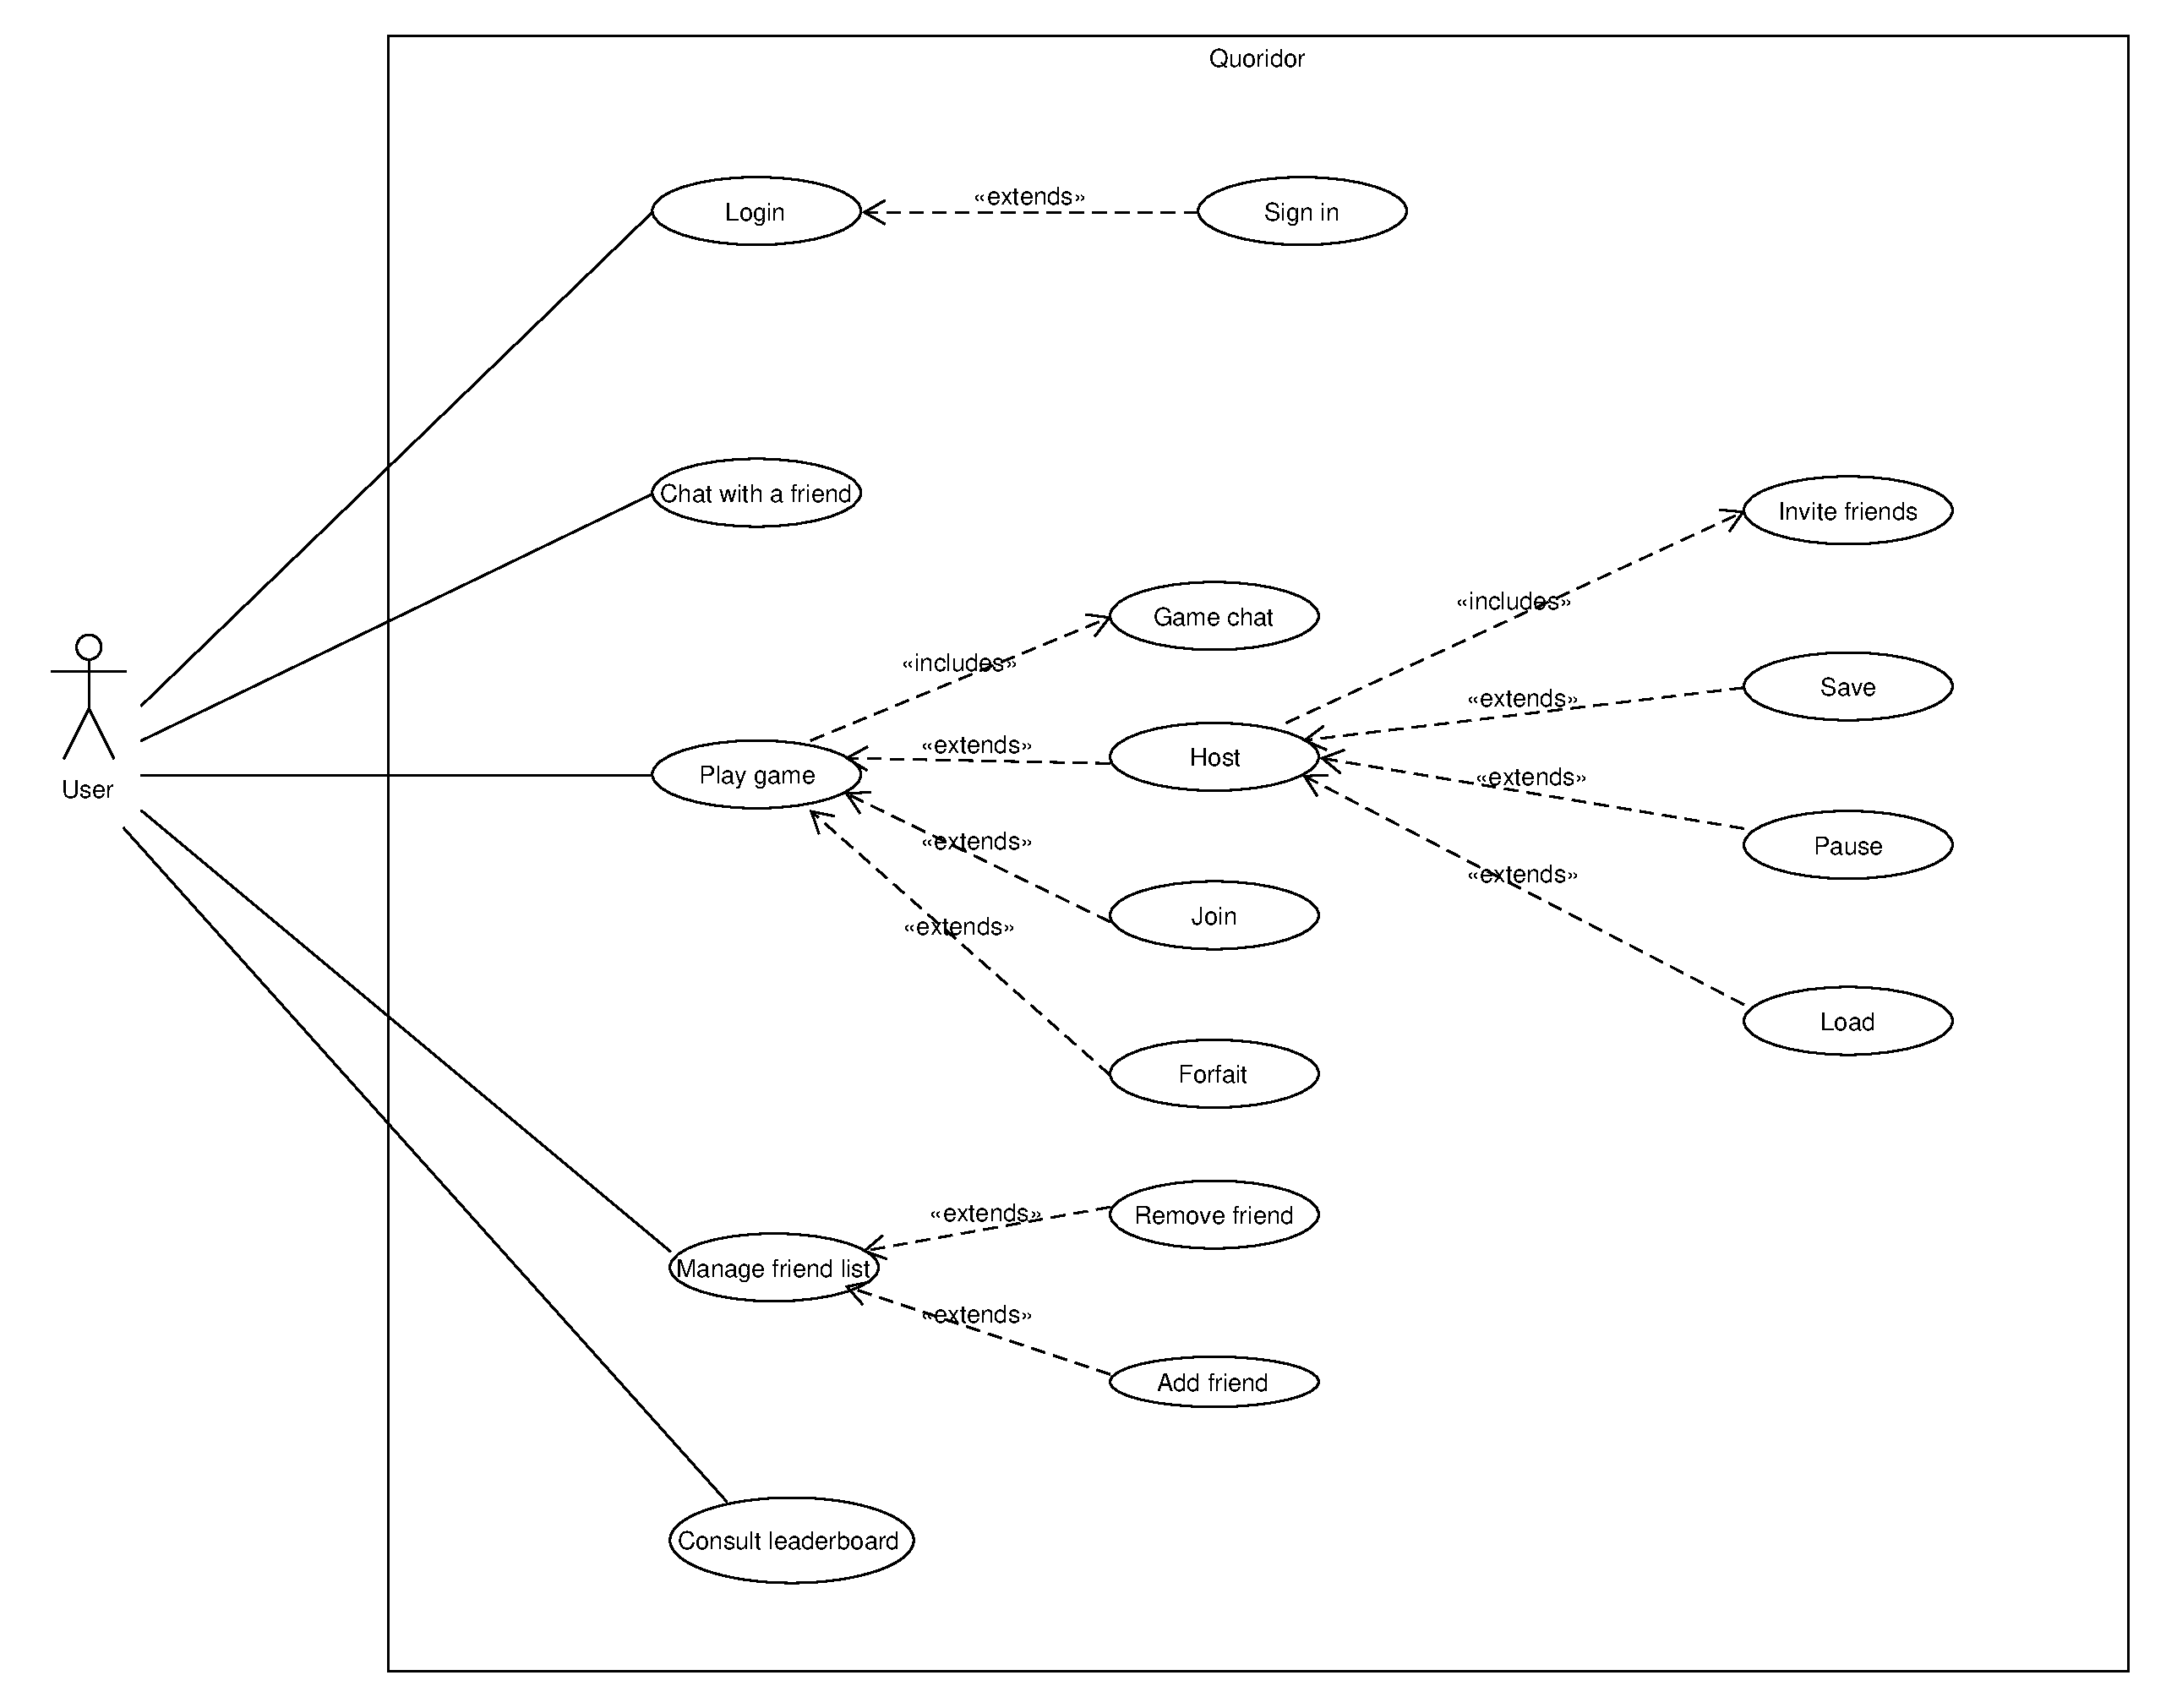
\includegraphics[width=5in]{use/main.pdf}
	\caption{Use Case}
	
	
\end{figure}

\subsubsection{Connexion}
\noindent
\begin{table}[H]
\begin{tabular}{|p{3cm}|p{3cm}|p{3cm}|p{3cm}|p{3cm}|}
\hline
	\textbf{Acteur} & \textbf{Pré-conditions} & \textbf{Post-conditions} & \textbf{Cas général}& \textbf{Cas exceptionnels} \\
\hline
	Log in & L'utilisateur possède déjà un compte & L'utilisateur est connecté & L'utilisateur indique son nom d'utilisateur et son mot de passe& Nom d'utilisateur incorrect

	Mot de passe incorrect \\
\hline
	Sign in & L'utilisateur n'a pas de compte & L'utilisateur a créé un compte & L'utilisateur entre un nom d'utilisateur et deux fois son mot de passe& Le nom d'utilisateur existe déjà

Le mot de passe ne respecte pas les conditions\\
\hline
\end{tabular}
	\caption{Use case: explications du mécanisme de connexion et de création de compte}
\end{table}
\subsubsection{Gestion des amis}
\noindent

\begin{table}[H]
\begin{tabular}{|p{3.5cm}|p{3cm}|p{3cm}|p{3cm}|p{3cm}|}
\hline
\textbf{Acteur} & \textbf{Pré-conditions} & \textbf{Post-conditions} & \textbf{Cas général}& \textbf{Cas exceptionnels} \\
\hline
Chat with friend& 
L'utilisateur doit avoir l'ami avec lequel il veut communiquer dans sa liste d'amis

L'ami doit être connecté& L'utilisateur a envoyé un message à un ami & L'utilisateur envoie un message à l'ami de son choix & Néant \\
\hline
	Consult leaderboard & L'utilisateur doit être connecté & Néant & L'utilisateur consulte le tableau des scores & Néant \\
\hline
Add friend & L'ami possède un compte& Néant & L'ami est ajouté dans la liste d'amis de l'utilisateur & L'utilisateur est déjà ami avec cette personne\\ \hline
Remove friend& L'utilisateur connecté doit cibler un ami & Néant & L'ami cible est retiré de la liste& Néant\\
\hline
\end{tabular}
	\caption{Use case: explications de la gestion des amis}
\end{table}
\subsubsection{Lancement de partie}
\noindent

\begin{table}[H]
\begin{tabular}{|p{3.5cm}|p{3cm}|p{3cm}|p{3cm}|p{3cm}|}
\hline
\textbf{Acteur} & \textbf{Pré-conditions} & \textbf{Post-conditions} & \textbf{Cas général}& \textbf{Cas exceptionnels} \\
\hline
Host Game & L'utilisateur doit être connecté

	L'utilisateur ne doit pas se trouver en partie& Néant  & L'utilisateur peut choisir les modes de jeu et inviter des amis & Néant\\
\hline


	
Load & Être host de la partie en cours & Neant & Une partie est antérieurement sauvegardée est chargée & Fichier de sauvegarde incompatible\\
\hline
Invite friends & Être host de la partie en cours

Avoir des amis connectés dans sa liste d'amis 
& L'ami a le choix d'accepter ou de refuser une invitation & Les amis sont invités à rejoindre une partie & L'ami invité est déjà dans une partie.\\
\hline
Join Game &
	L'utilisateur doit être connecté

	L'utilisateur ne doit pas se trouver en partie

	L'utilisateur doit avoir accepté une invitation & Néant  & L'utilisateur rejoint une partie & L'utilisateur tente de rejoindre une partie déjà pleine\\
\hline
Play Game& Le nombre de joueurs présents est 2 ou 4 & Néant  & L'utilisateur joue une partie avec ses amis & Néant\\
\hline


\end{tabular}
	\caption{Use case: explications du mécanisme de création de partie}
\end{table}
\subsubsection{Partie de jeu}
\begin{table}[H]
\begin{tabular}{|p{3.5cm}|p{3cm}|p{3cm}|p{3cm}|p{3cm}|}
\hline
\textbf{Acteur} & \textbf{Pré-conditions} & \textbf{Post-conditions} & \textbf{Cas général}& \textbf{Cas exceptionnels} \\
\hline
Save & Être host de la partie en cours et l'avoir mise en pause & Néant  & La partie est sauvegardée dans un fichier & Néant\\
\hline
Forfeit & Être en partie & L'utilisateur n'est plus présent dans une partie & L'utilisateur a perdu &Néant\\
\hline
Pause & Être host de la partie en cours & Les joueurs ne peuvent pas interagir pour le moment& La partie se met en pause & Néant\\
\hline
	Game chat & Être en partie & Néant & Permet de parler avec les joueurs de la partie en cours & Le message est trop volumineux\\
\hline

\end{tabular}
	\caption{Use case: explications des fonctionnalités disponibles lors de la partie de jeu}
\end{table}


\newpage

\subsection{Diagrammes de classe}

\begin{figure}[H]
	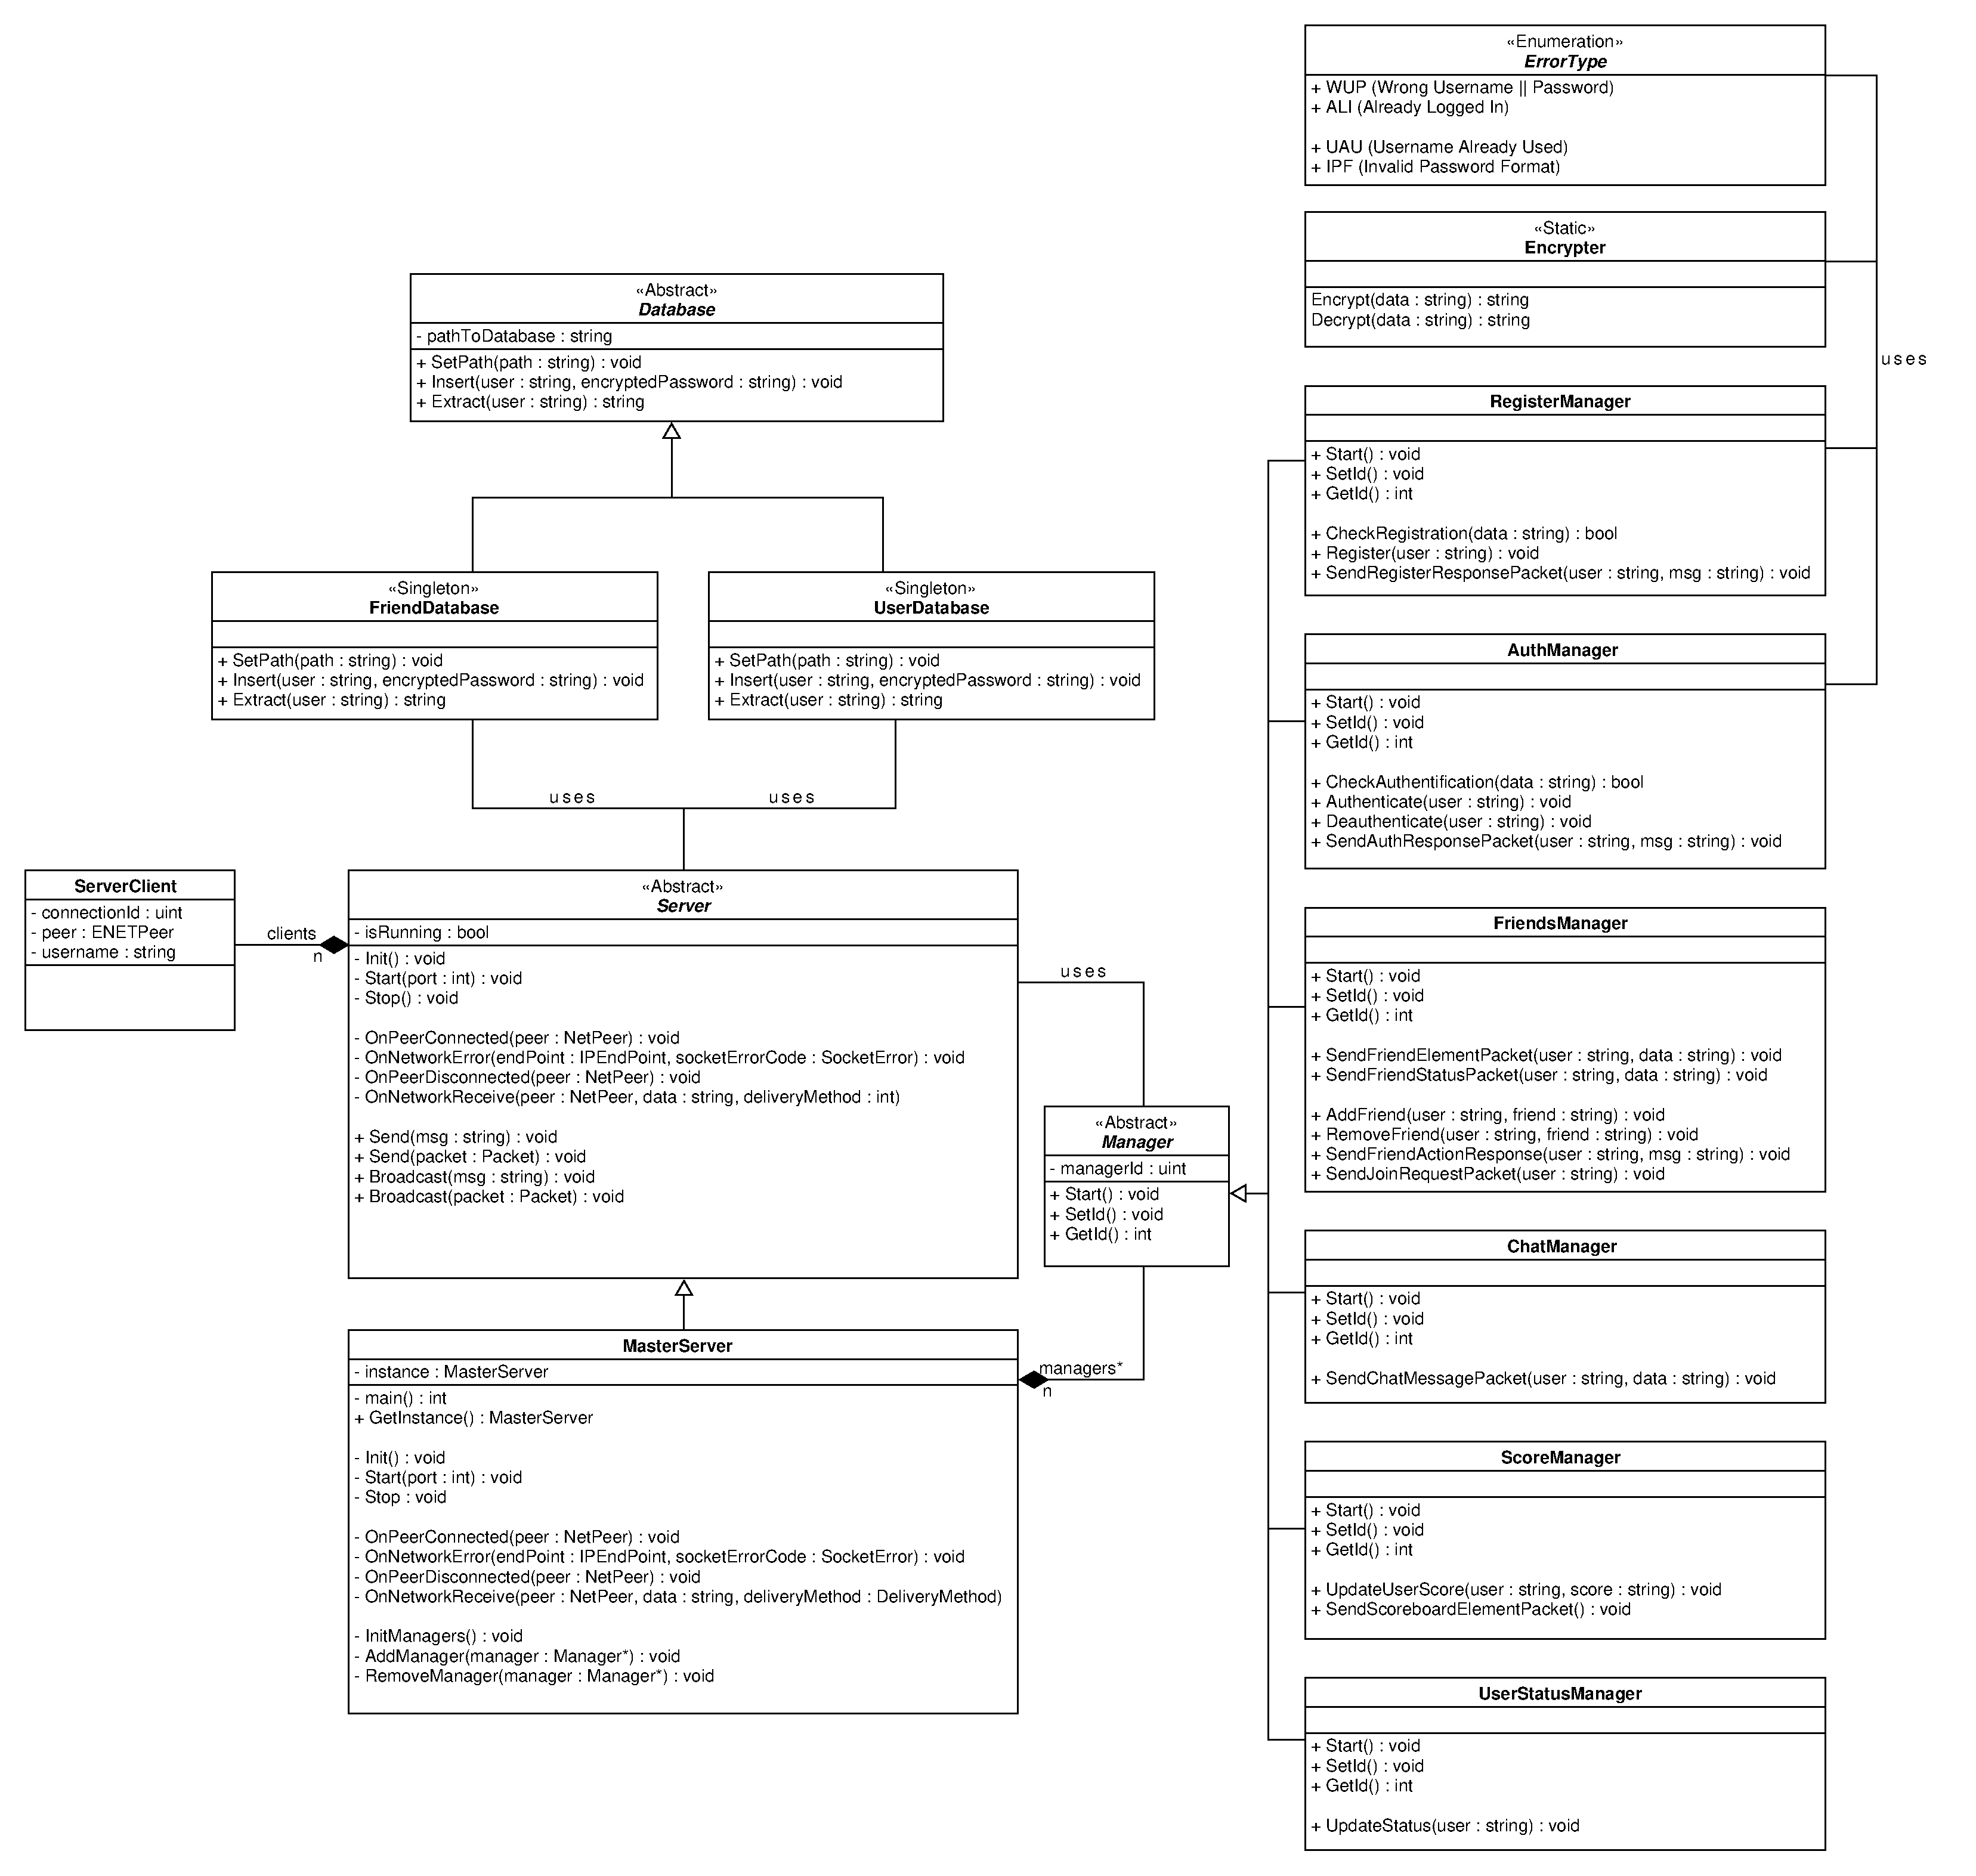
\includegraphics[width=7in]{class/master-server.pdf}
	\caption{Diagramme de classe :\textit{ master server}}
	
\end{figure}
\cmd{MasterServer} gère l'authentification, l'enregistrement, les invitations de parties, les amis ainsi que le chat entre joueurs.
\cmd{Manager} Plug-in lancé par le \cmd{MasterServer} permetant de gérer un tâche spécifique.
\begin{figure}[H]
	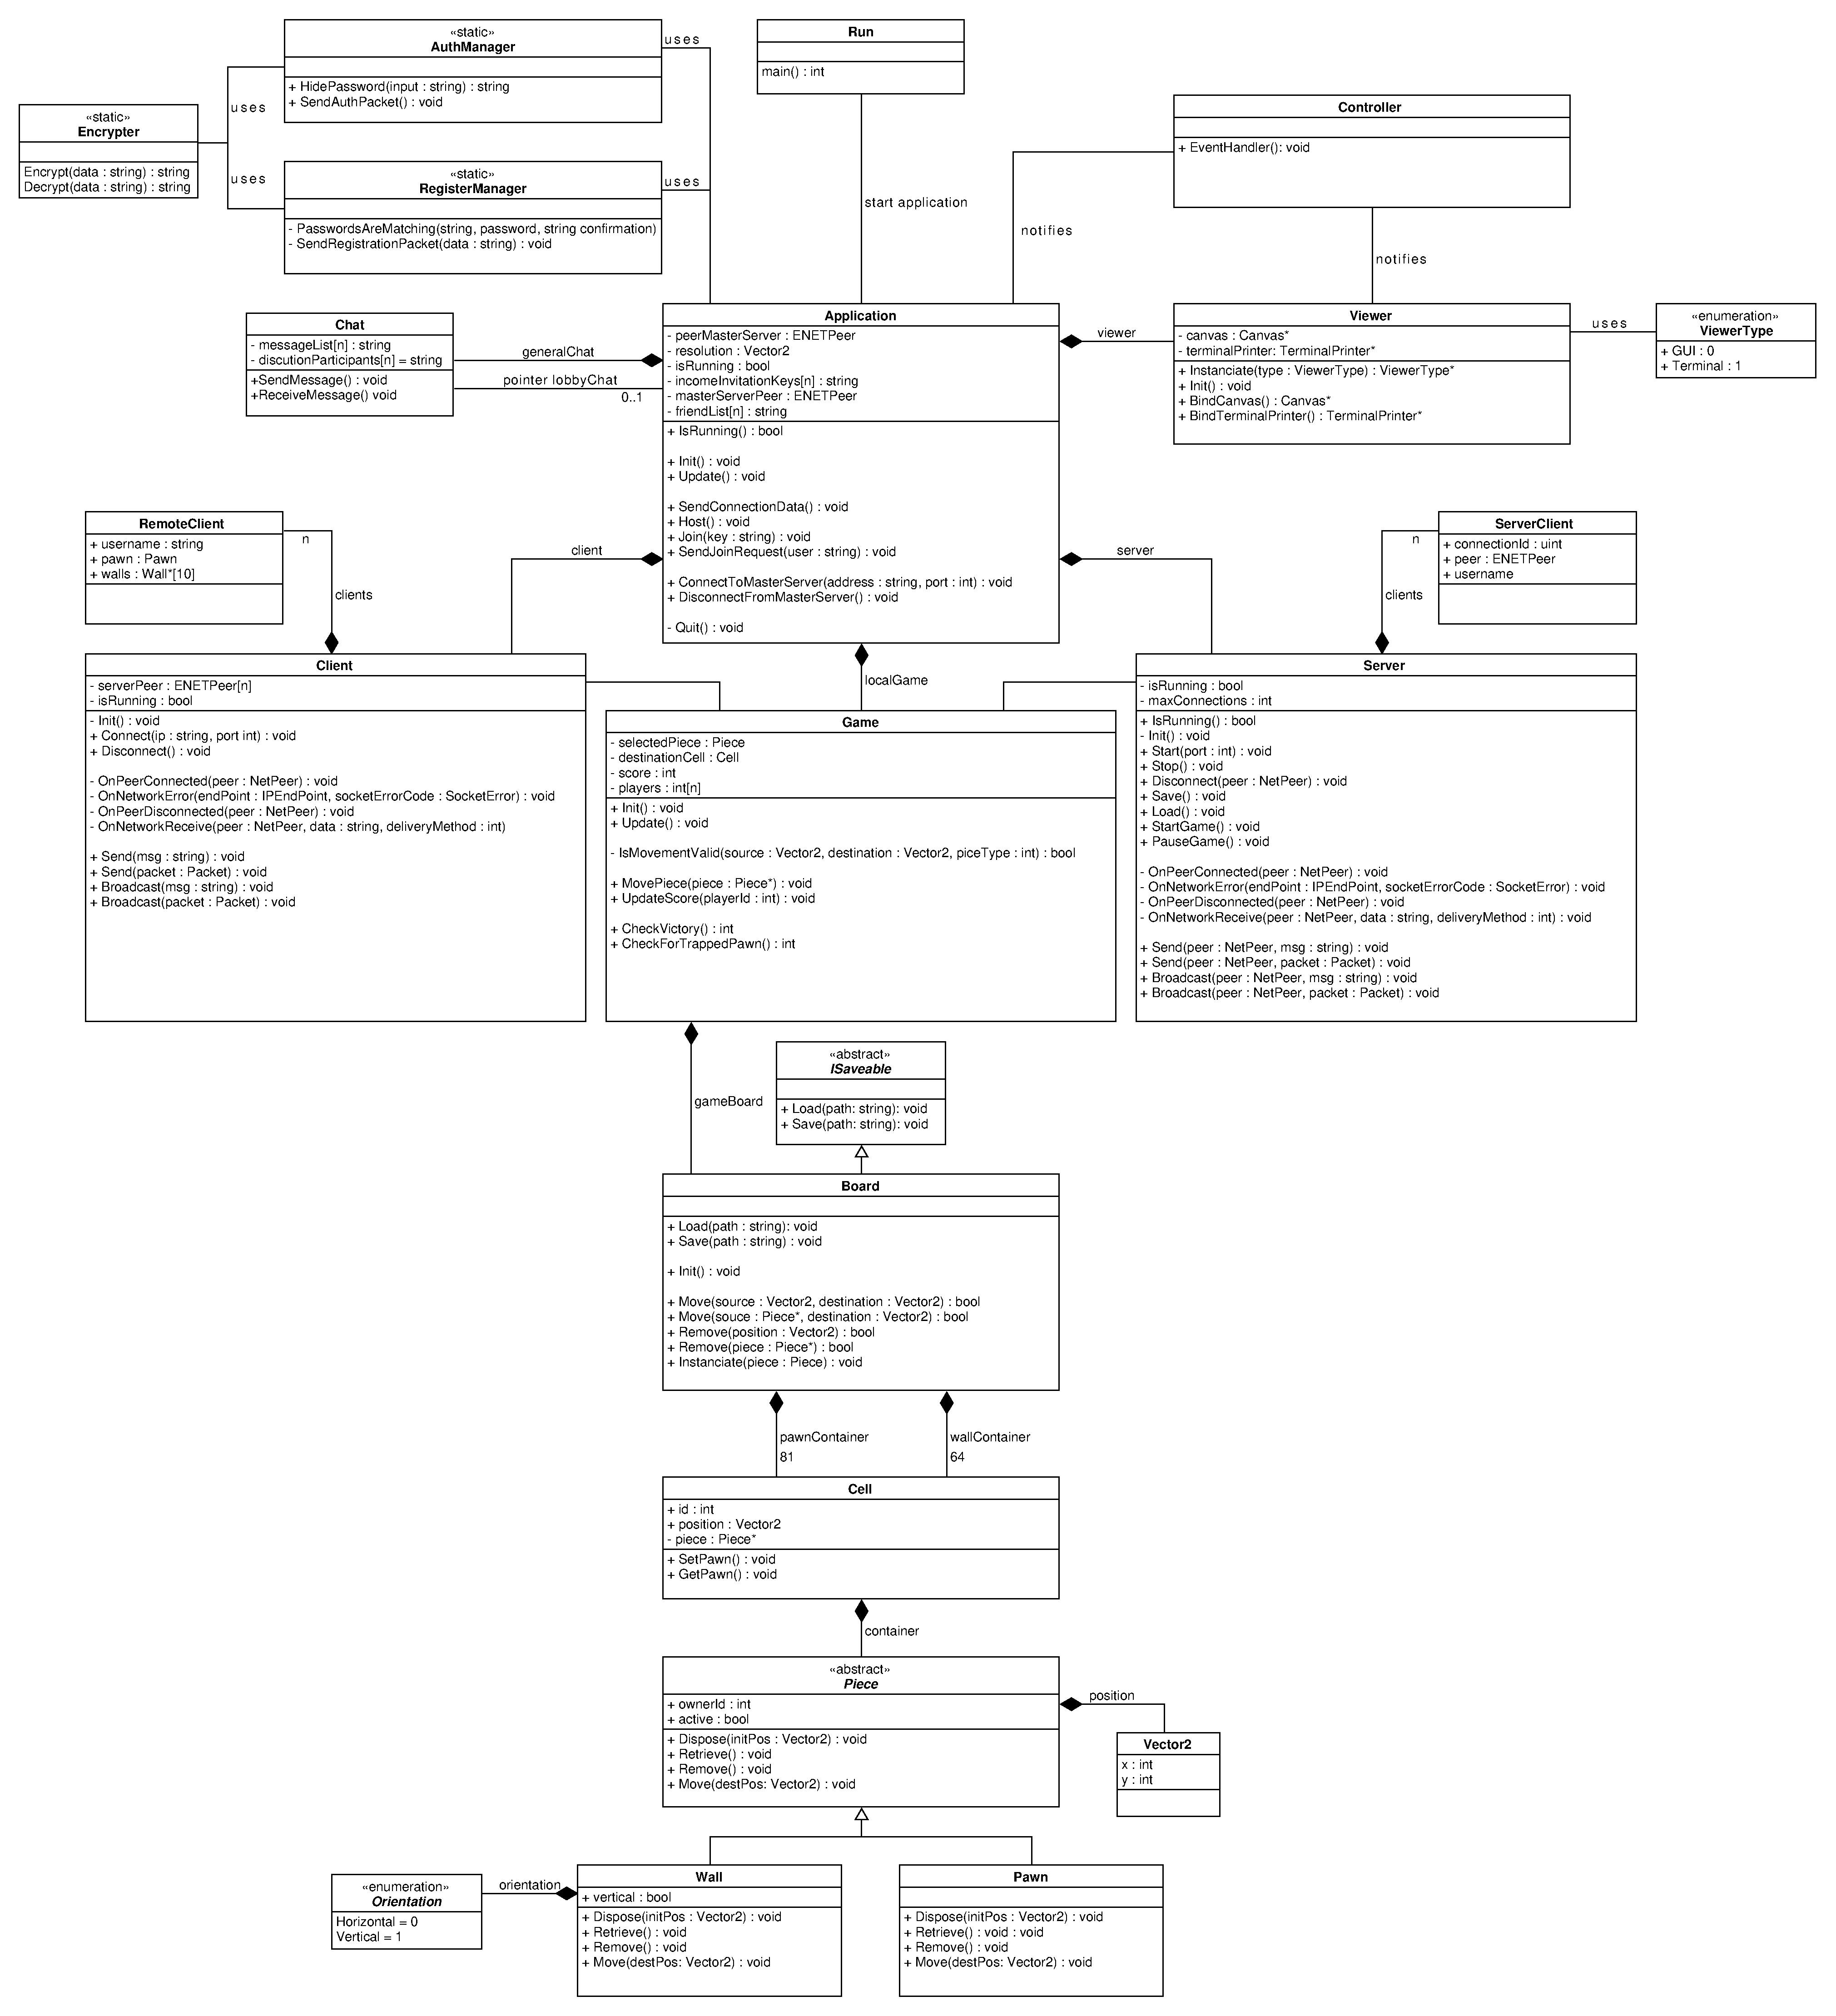
\includegraphics[width=7in]{class/application.pdf}
	\caption{Diagramme de classe : Application}
\end{figure}


\cmd{Application} est la classe principale qui gère tout le programme. Elle s'occupe de la communication avec le \textit{master server}, de l'interface graphique, le reseau (client et serveur) et se charge de lancer le jeu.

\cmd{Encrypter} permet de chiffrer et déchiffrer un message.
\cmd{AuthManager} s'occupe de l'authentification à l'aide d'\cmd{Encrypter} et de l'envoi'authentification au \textit{master server}.
\cmd{RegisterManager} s'occupe de la création d'un compte et de l'envoi de ces données au \textit{master server}.

\cmd{Chat} s'occupe de l'envoi et de la réception des messages des messages, et des utilisateurs ayant accès au chat.

\cmd{Client} représente la partie réseau de l'utilisateur qui n'est pas \textit{host}. Il peut se connecter, se déconnecter du serveur (hebergé par le host), d'envoyer et de recevoir des informations depuis le réseau.
\cmd{RemoteClient} est la représentation des autres clients pour un client.

\cmd{Server} représente la partie réseau du \textit{host} mais pas seulement. Il s'occupe aussi de lancer le serveur de la partie, envoie et reçois des informations des clients. 
\cmd{ServerClient} est la représentation des clients pour le client.

\cmd{Game} représente la logique du jeu. Il gère le tour des joueurs, les coups, les défaites et la victoire.

\cmd{Board} représente la structure du plateau.

\cmd{Board} représente le plateau dans le jeu.
\cmd{Wall} représente un mur, son état et ses actions dans le jeu.
\cmd{Pawn} représente un pion, son état et ses actions dans le jeu.
\cmd{Cell} est le conteneur des {Piece}
\cmd{Controller} permet à l'utilisateur de controller.

\begin{figure}[H]
	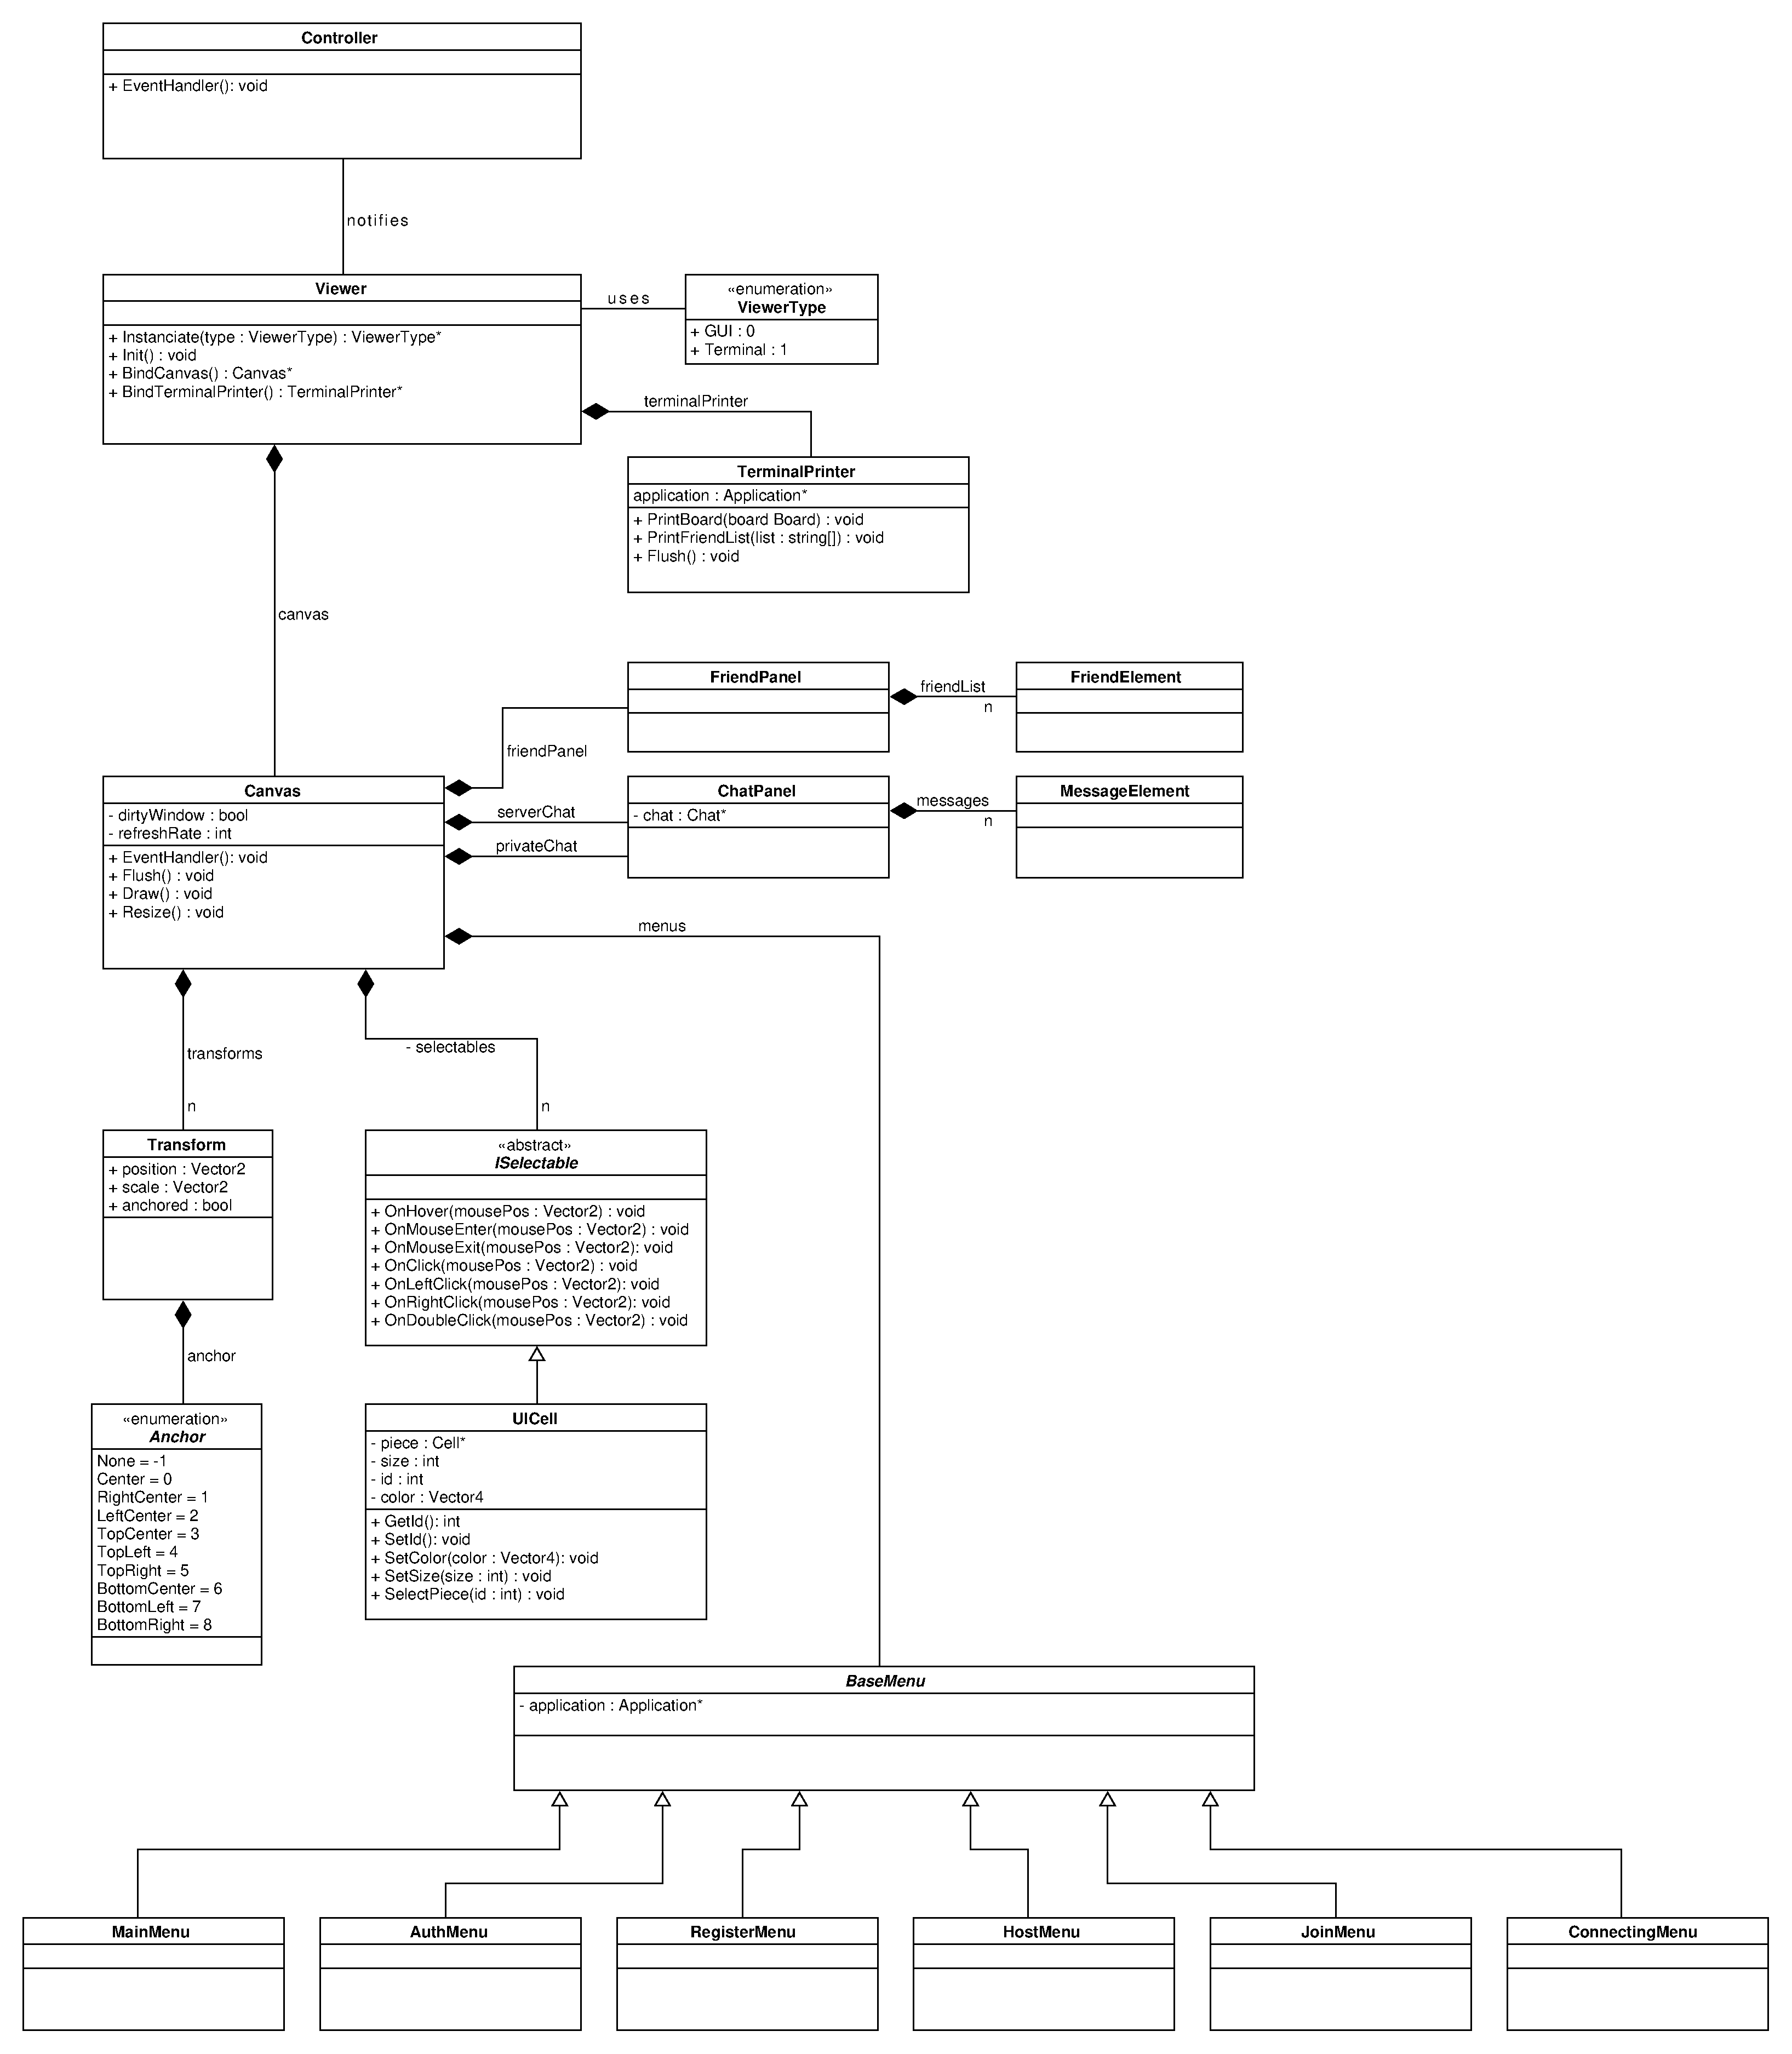
\includegraphics[width=7in]{class/interface.pdf}
	\caption{Diagramme de classe : Interface}
\end{figure}
 \cmd{Viewer} permet à l'utilisateur de voir une representation de l'application via une interface.
\cmd{TerminalPrinter} Gère l'interface terminal.
\cmd{Canvas} Gère l'interface graphique GUI.

\subsection{Diagrammes de séquence}

\begin{figure}[H]
	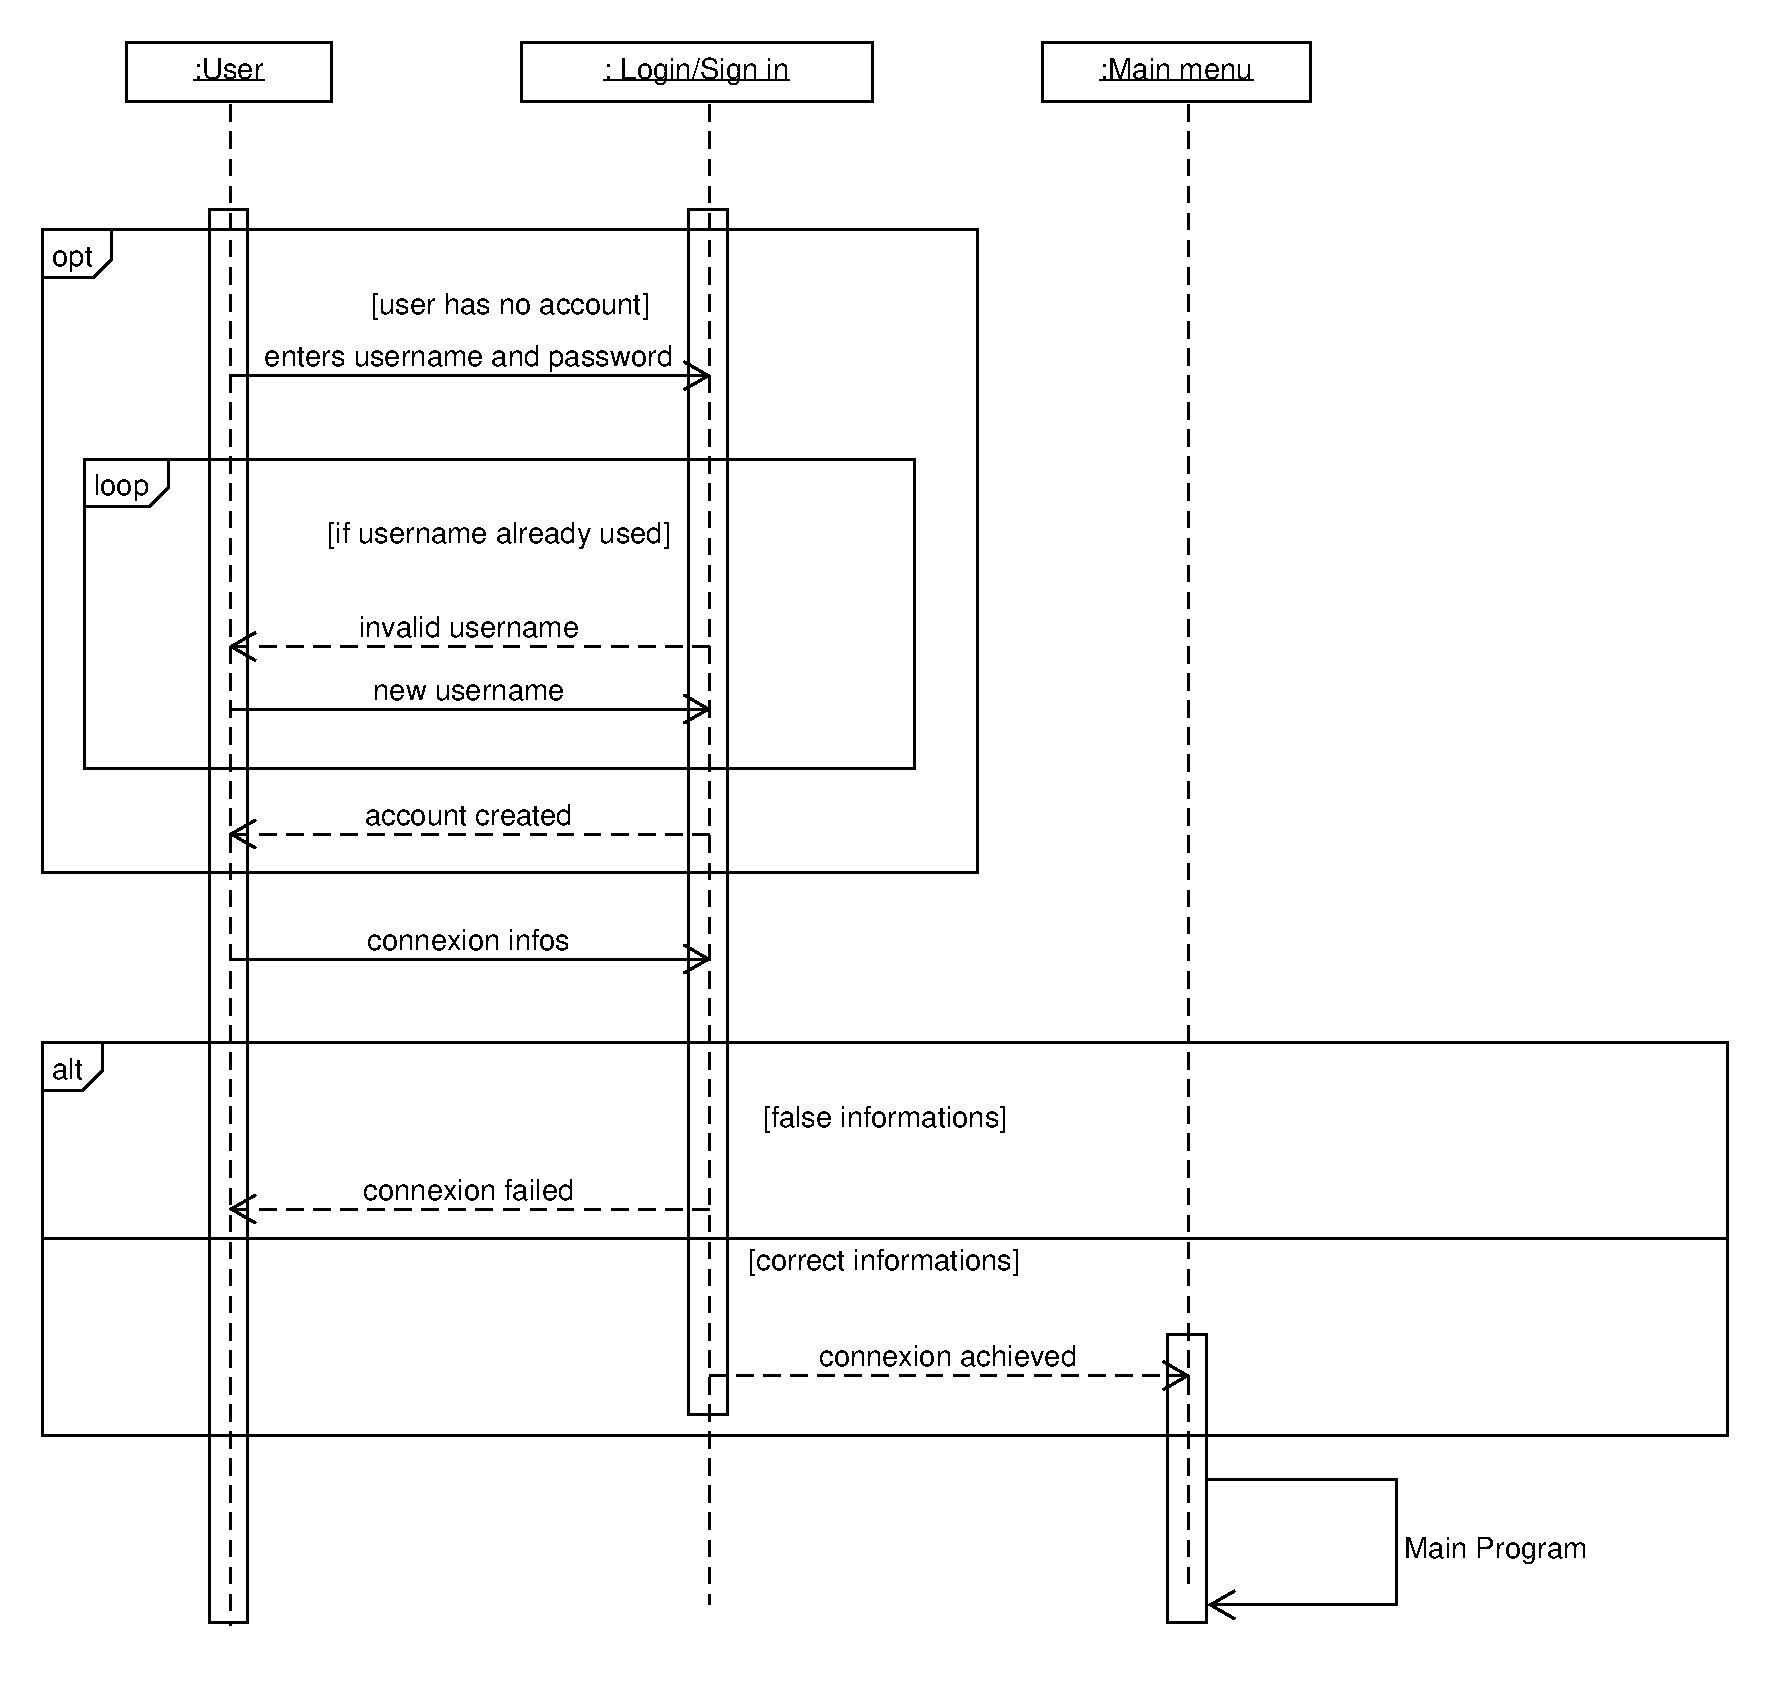
\includegraphics[width=6in]{sequence/connection.pdf}
	\caption{Diagramme de séquence : Connexion}
\end{figure}


\begin{figure}[H]

	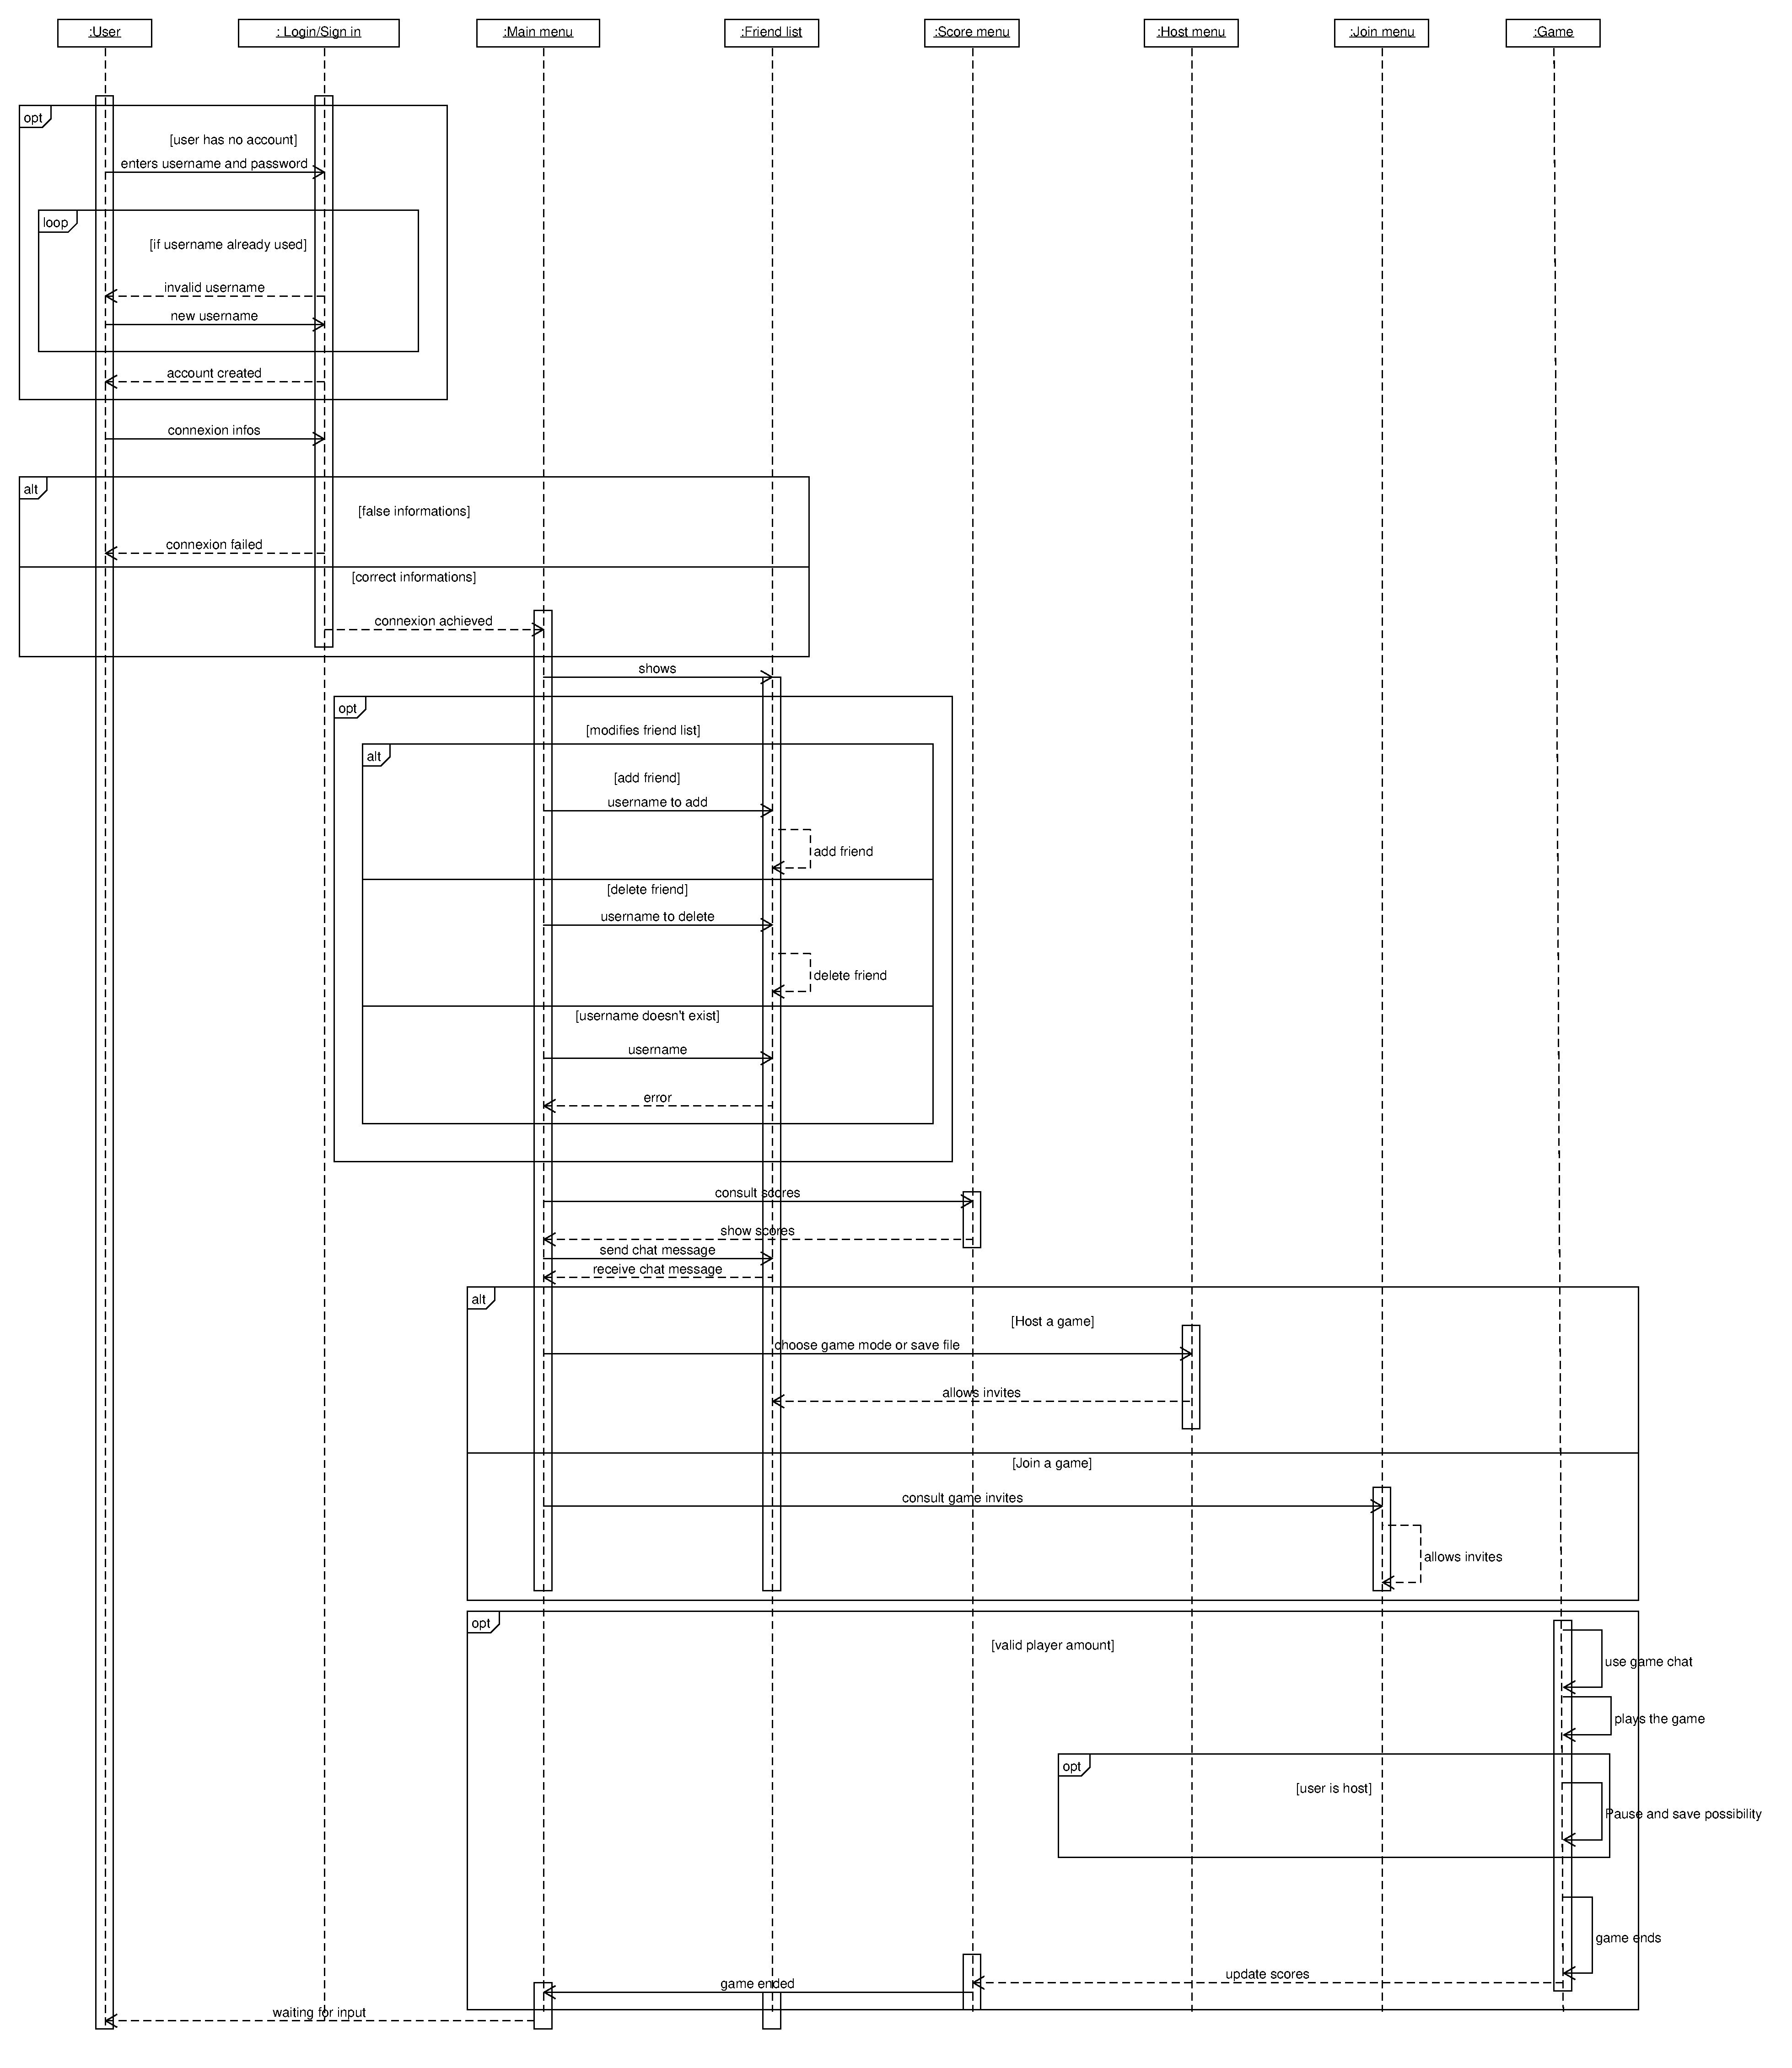
\includegraphics[width=6in]{sequence/menu.pdf}
	\caption{Diagramme de séquence : Principal}
\end{figure}

\begin{figure}[H]
	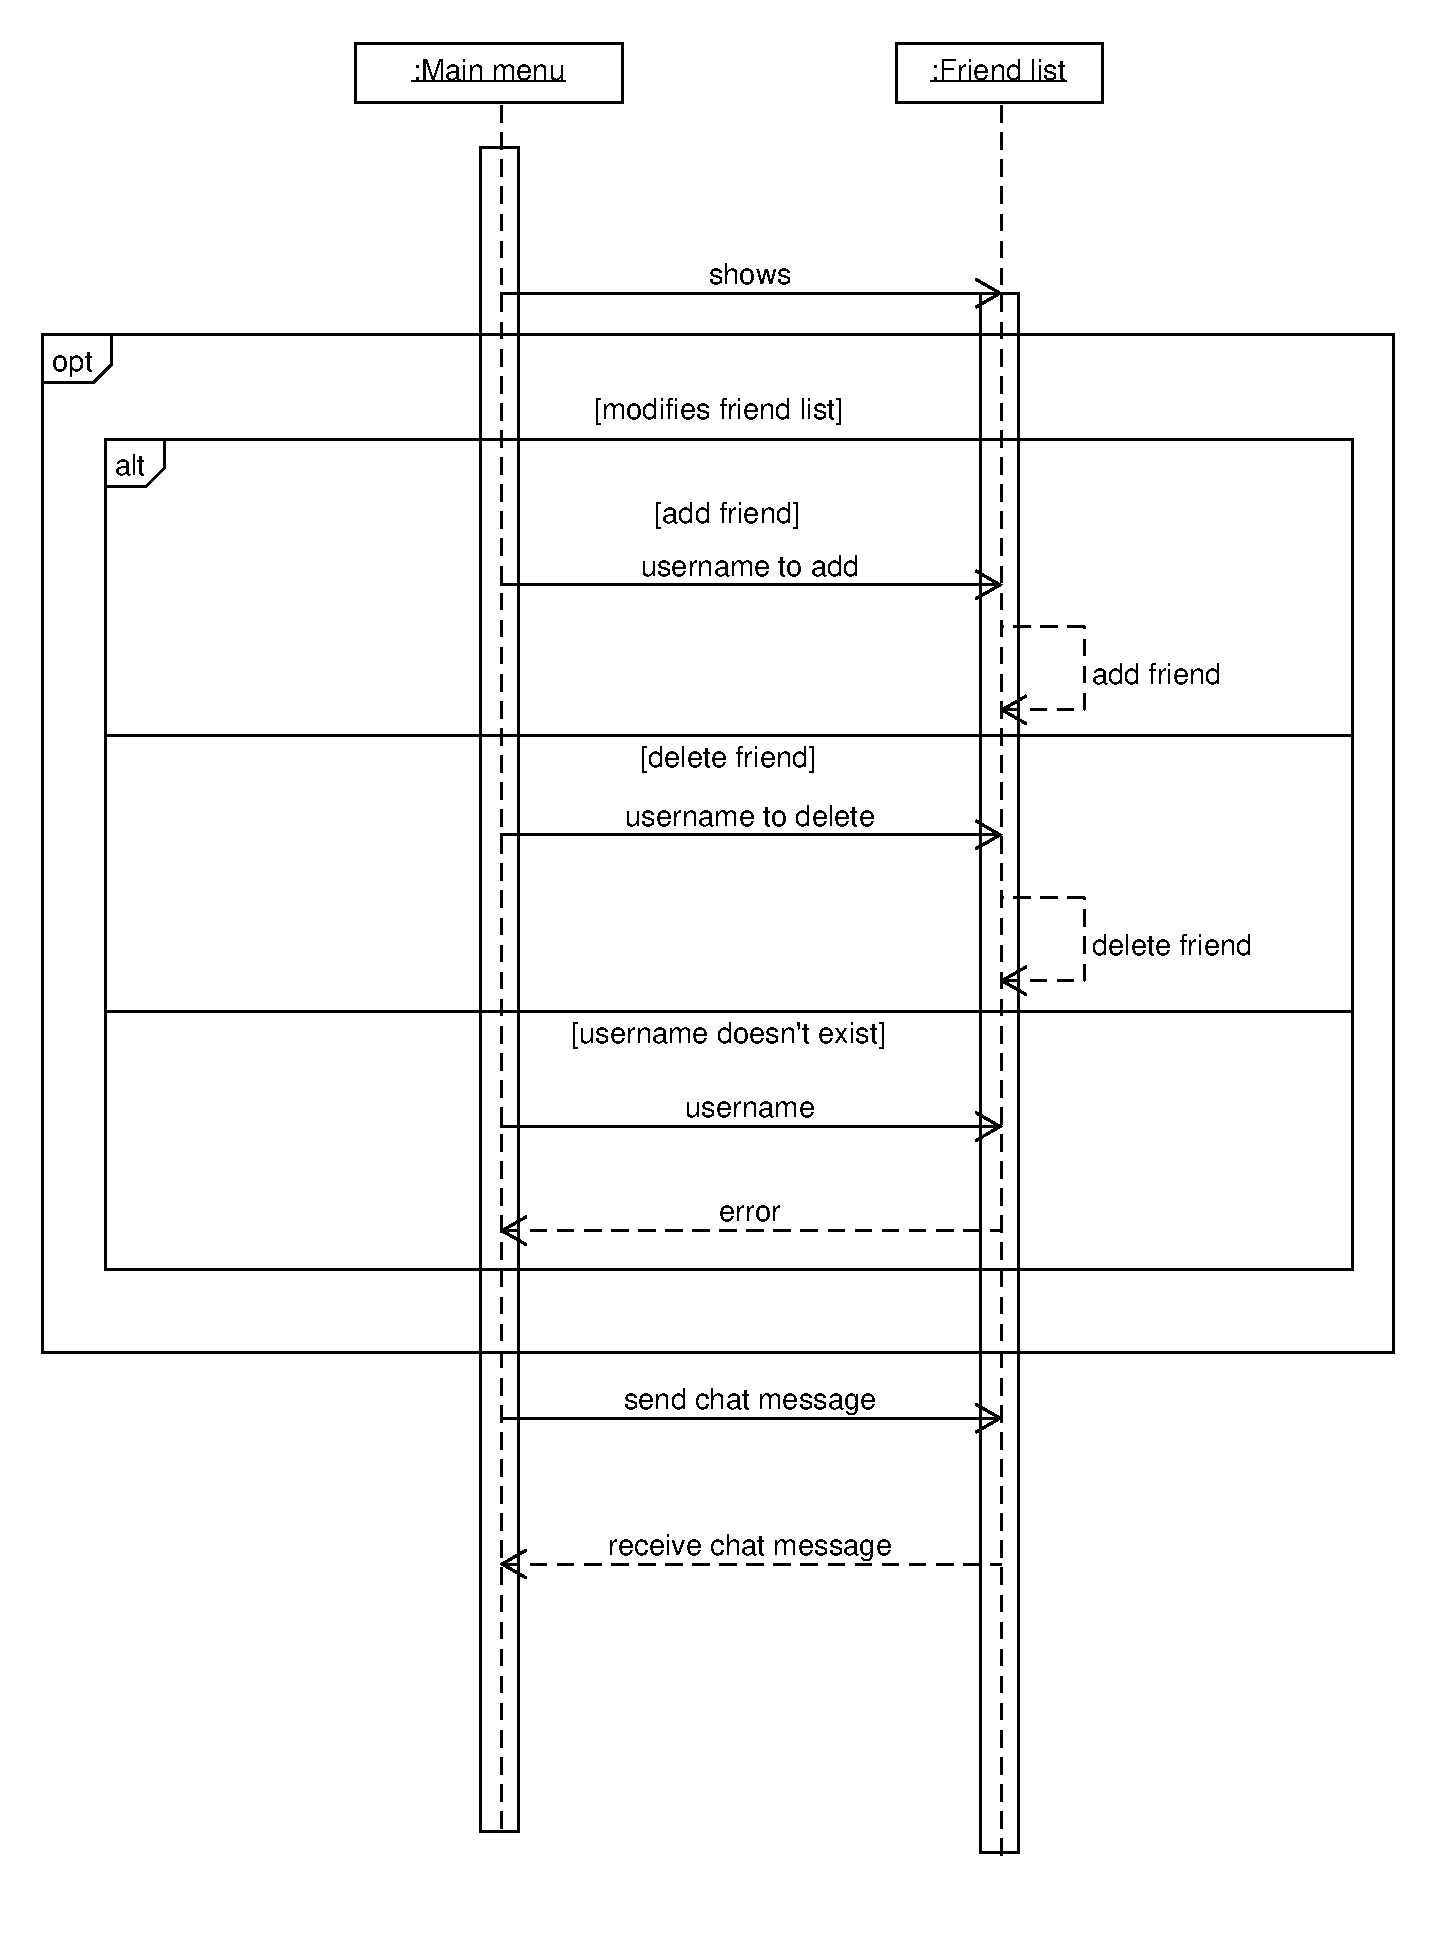
\includegraphics[width=6in]{sequence/friends.pdf}
	\caption{Diagramme de séquence : Amis}
\end{figure}


\begin{figure}[H]
	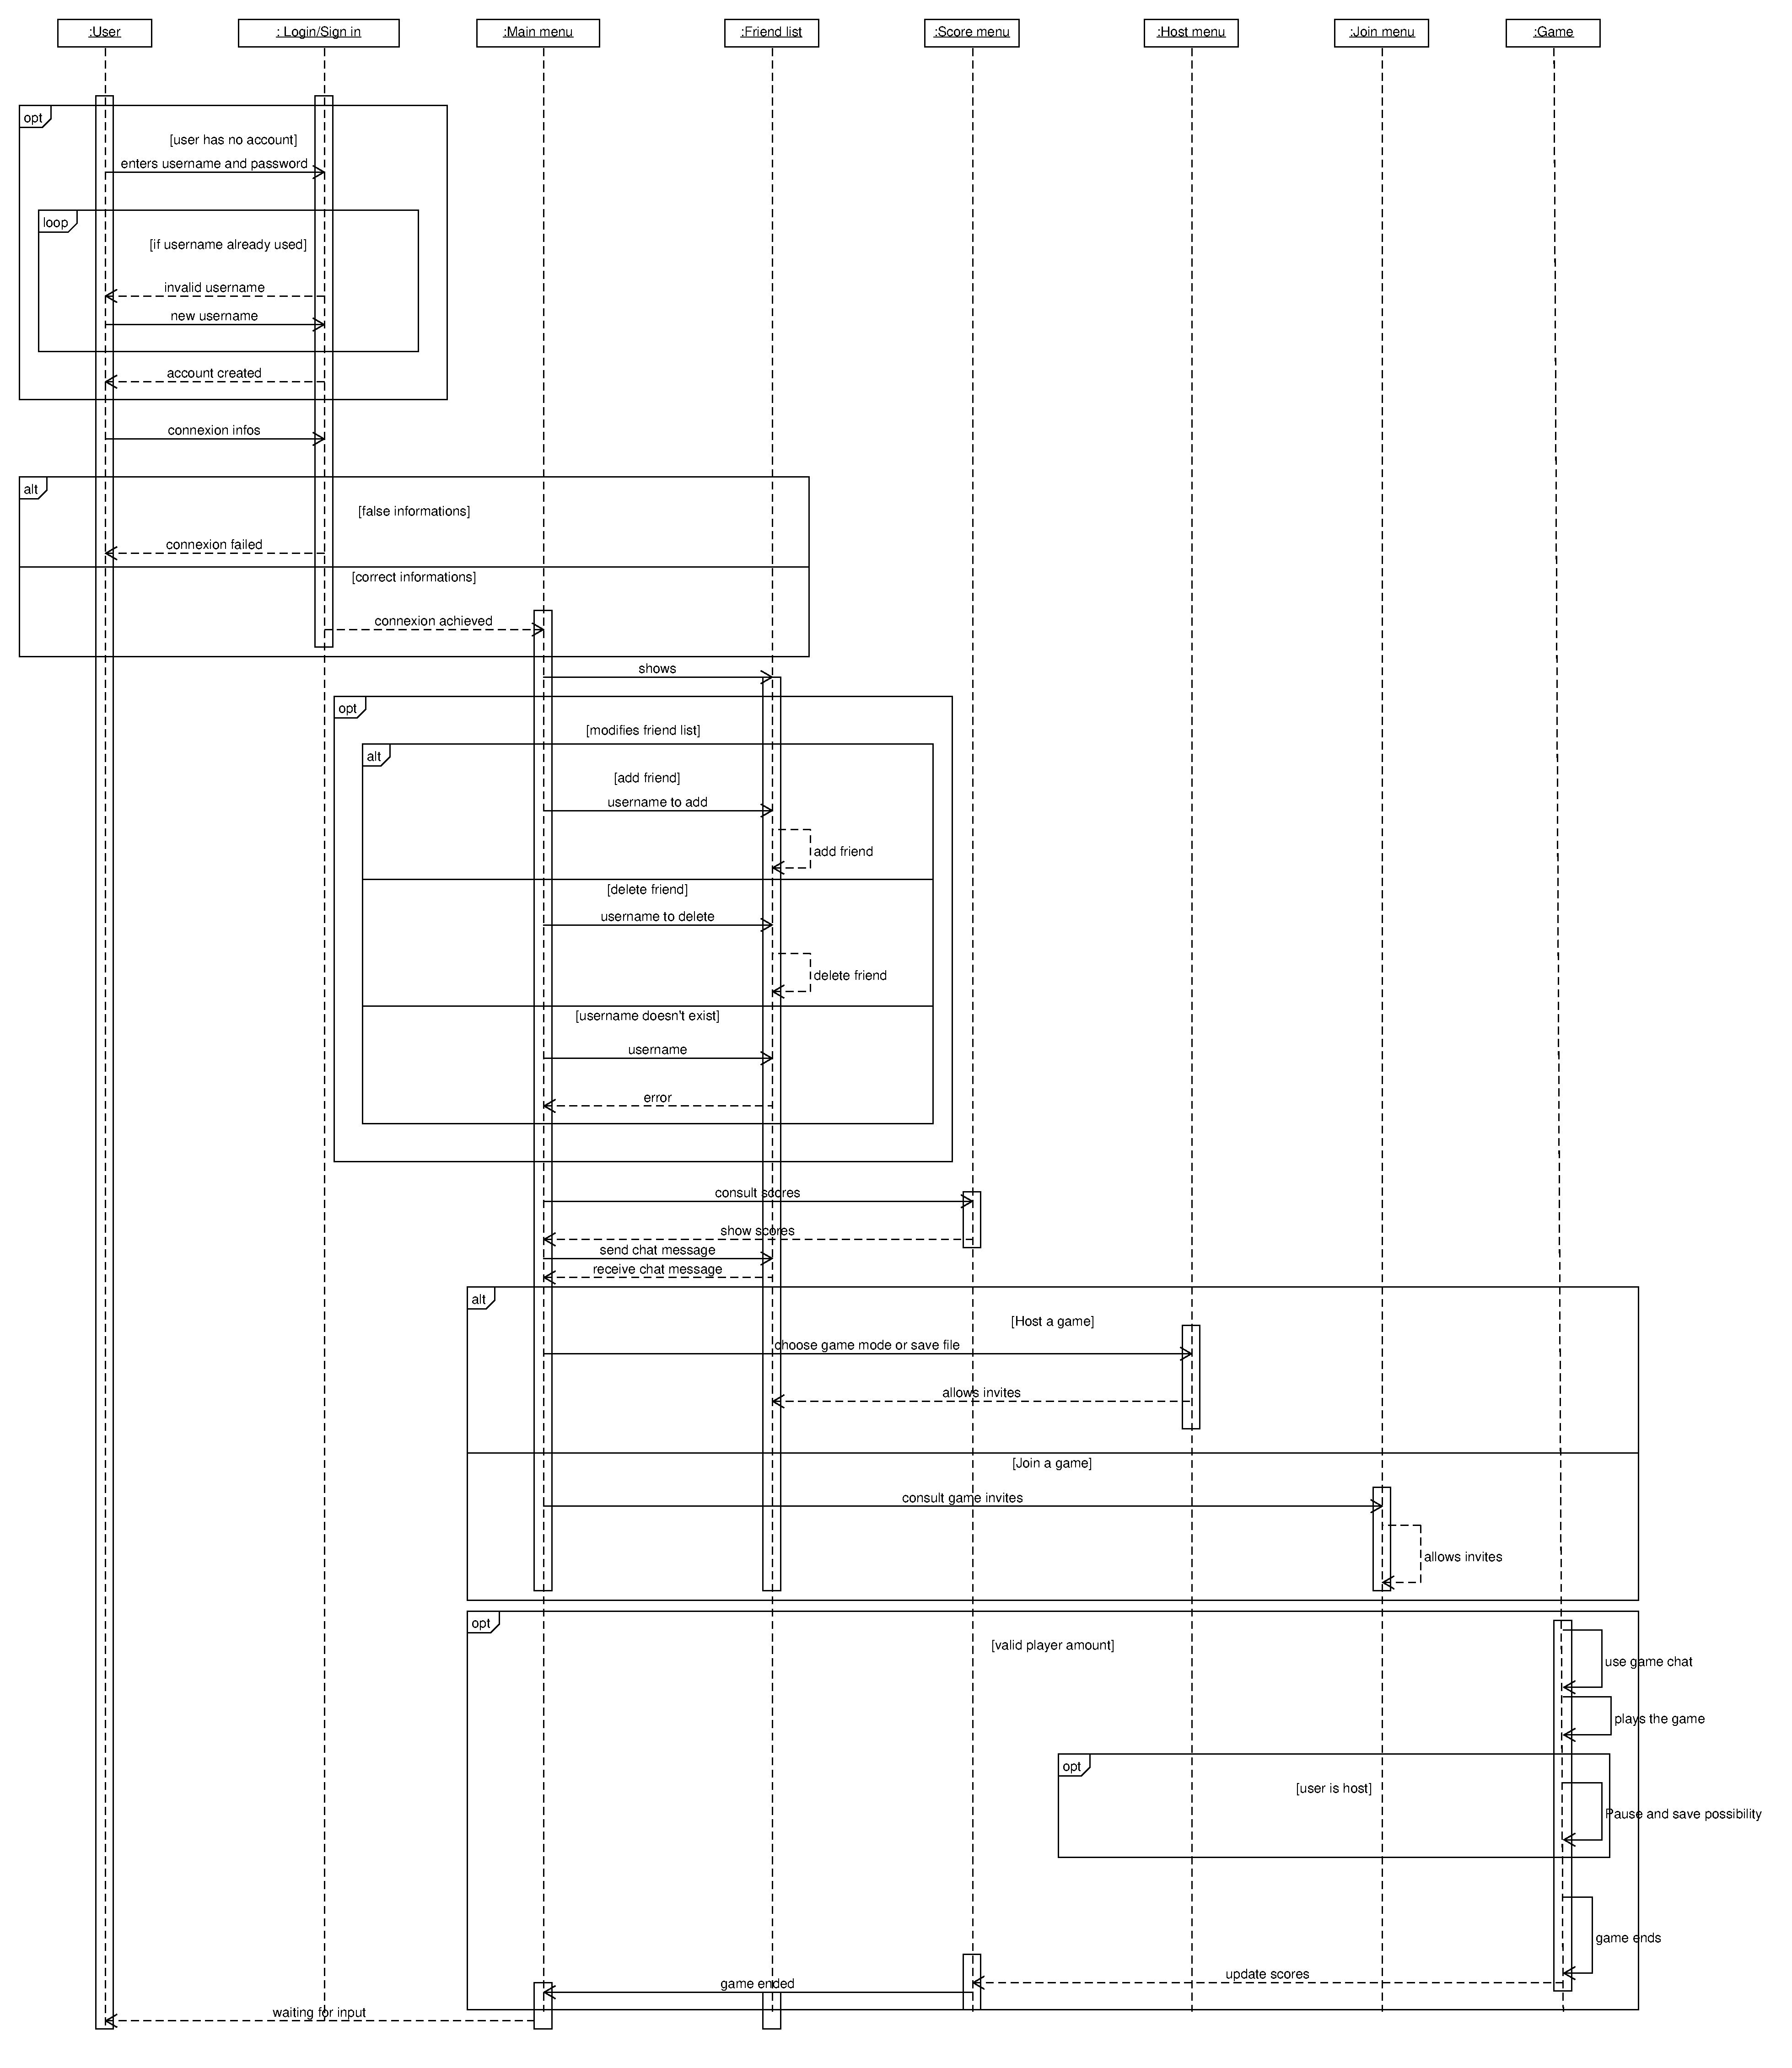
\includegraphics[width=6in]{sequence/game.pdf}
	\caption{Diagramme de séquence : Jeu}
\end{figure}






\newpage
\subsection{Exemple d'interface}
\begin{figure}[H]
	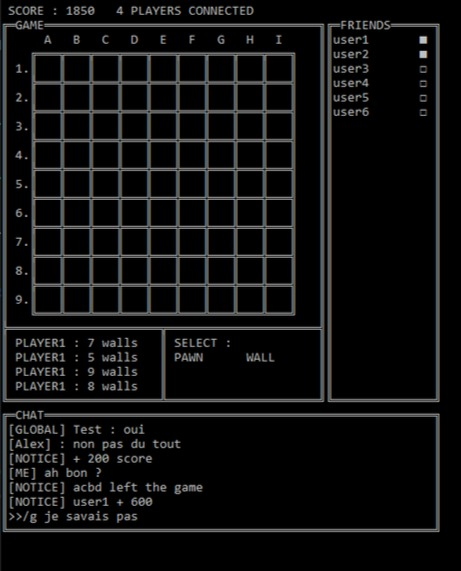
\includegraphics[width=6in]{images/terminal-example.jpg}\\
	\caption{Exemple design de la partie en terminal}
\end{figure}
\newpage




\end{document}

%réajuster le use case pour que l'utilisateur soit plus proche de jouer.
%éparer le class diagram en parties reseau - partie etc

